%% LyX 2.2.3 created this file.  For more info, see http://www.lyx.org/.
%% Do not edit unless you really know what you are doing.
\documentclass[ruled]{article}
\usepackage{courier}
\usepackage[T1]{fontenc}
\usepackage[latin9]{inputenc}
\usepackage[letterpaper]{geometry}
\geometry{verbose}
\usepackage{color}
\usepackage{url}
\usepackage{algorithm2e}
\usepackage{amsmath}
\usepackage{amssymb}
\usepackage{titlesec}
%\newcommand{\sectionbreak}{\clearpage}
\usepackage{graphicx}
\usepackage[export]{adjustbox}
\graphicspath{ {./images/} }
\usepackage{listings}
\usepackage{pdfpages}
\usepackage[unicode=true,
 bookmarks=false,
 breaklinks=false,pdfborder={0 0 1},backref=section,colorlinks=true]
 {hyperref}

\makeatletter

%%%%%%%%%%%%%%%%%%%%%%%%%%%%%% LyX specific LaTeX commands.
\providecommand{\LyX}{\texorpdfstring%
  {L\kern-.1667em\lower.25em\hbox{Y}\kern-.125emX\@}
  {LyX}}
%% Special footnote code from the package 'stblftnt.sty'
%% Author: Robin Fairbairns -- Last revised Dec 13 1996
\let\SF@@footnote\footnote
\def\footnote{\ifx\protect\@typeset@protect
    \expandafter\SF@@footnote
  \else
    \expandafter\SF@gobble@opt
  \fi
}
\expandafter\def\csname SF@gobble@opt \endcsname{\@ifnextchar[%]
  \SF@gobble@twobracket
  \@gobble
}
\edef\SF@gobble@opt{\noexpand\protect
  \expandafter\noexpand\csname SF@gobble@opt \endcsname}
\def\SF@gobble@twobracket[#1]#2{}

\@ifundefined{date}{}{\date{}}
%%%%%%%%%%%%%%%%%%%%%%%%%%%%%% User specified LaTeX commands.
\definecolor{mygreen}{rgb}{0,0.6,0}
\definecolor{mygray}{rgb}{0.5,0.5,0.5}
\definecolor{mymauve}{rgb}{0.58,0,0.82}

\makeatother

\usepackage{listings}
\lstset{backgroundcolor={\color{white}},
basicstyle={\footnotesize\ttfamily},
breakatwhitespace=false,
breaklines=true,
captionpos=b,
commentstyle={\color{mygreen}},
deletekeywords={...},
escapeinside={\%*}{*)},
extendedchars=true,
frame=shadowbox,
keepspaces=true,
keywordstyle={\color{blue}},
language=Python,
morekeywords={*,...},
numbers=none,
numbersep=5pt,
numberstyle={\tiny\color{mygray}},
rulecolor={\color{black}},
showspaces=false,
showstringspaces=false,
showtabs=false,
stepnumber=1,
stringstyle={\color{mymauve}},
tabsize=2}

 
\begin{document}

\global\long\def\reals{\mathbf{R}}
 \global\long\def\integers{\mathbf{Z}}
\global\long\def\naturals{\mathbf{N}}
 \global\long\def\rationals{\mathbf{Q}}
\global\long\def\ca{\mathcal{A}}
\global\long\def\cb{\mathcal{B}}
 \global\long\def\cc{\mathcal{C}}
 \global\long\def\cd{\mathcal{D}}
\global\long\def\ce{\mathcal{E}}
\global\long\def\cf{\mathcal{F}}
\global\long\def\cg{\mathcal{G}}
\global\long\def\ch{\mathcal{H}}
\global\long\def\ci{\mathcal{I}}
\global\long\def\cj{\mathcal{J}}
\global\long\def\ck{\mathcal{K}}
\global\long\def\cl{\mathcal{L}}
\global\long\def\cm{\mathcal{M}}
\global\long\def\cn{\mathcal{N}}
\global\long\def\co{\mathcal{O}}
\global\long\def\cp{\mathcal{P}}
\global\long\def\cq{\mathcal{Q}}
\global\long\def\calr{\mathcal{R}}
\global\long\def\cs{\mathcal{S}}
\global\long\def\ct{\mathcal{T}}
\global\long\def\cu{\mathcal{U}}
\global\long\def\cv{\mathcal{V}}
\global\long\def\cw{\mathcal{W}}
\global\long\def\cx{\mathcal{X}}
\global\long\def\cy{\mathcal{Y}}
\global\long\def\cz{\mathcal{Z}}
\global\long\def\ind#1{1(#1)}
\global\long\def\pr{\mathbb{P}}

\global\long\def\ex{\mathbb{E}}
\global\long\def\var{\textrm{Var}}
\global\long\def\cov{\textrm{Cov}}
\global\long\def\sgn{\textrm{sgn}}
\global\long\def\sign{\textrm{sign}}
\global\long\def\kl{\textrm{KL}}
\global\long\def\law{\mathcal{L}}
\global\long\def\eps{\varepsilon}
\global\long\def\convd{\stackrel{d}{\to}}
\global\long\def\eqd{\stackrel{d}{=}}
\global\long\def\del{\nabla}
\global\long\def\loss{\ell}
\global\long\def\tr{\operatorname{tr}}
\global\long\def\trace{\operatorname{trace}}
\global\long\def\diag{\text{diag}}
\global\long\def\rank{\text{rank}}
\global\long\def\linspan{\text{span}}
\global\long\def\proj{\text{Proj}}
\global\long\def\argmax{\operatornamewithlimits{arg\, max}}
\global\long\def\argmin{\operatornamewithlimits{arg\, min}}
\global\long\def\bfx{\mathbf{x}}
\global\long\def\bfy{\mathbf{y}}
\global\long\def\bfl{\mathbf{\lambda}}
\global\long\def\bfm{\mathbf{\mu}}
\global\long\def\calL{\mathcal{L}}
\global\long\def\vw{\boldsymbol{w}}
\global\long\def\vx{\boldsymbol{x}}
\global\long\def\vxi{\boldsymbol{\xi}}
\global\long\def\valpha{\boldsymbol{\alpha}}
\global\long\def\vbeta{\boldsymbol{\beta}}
\global\long\def\vsigma{\boldsymbol{\sigma}}
\global\long\def\vmu{\boldsymbol{\mu}}
\global\long\def\vtheta{\boldsymbol{\theta}}
\global\long\def\vd{\boldsymbol{d}}
\global\long\def\vs{\boldsymbol{s}}
\global\long\def\vt{\boldsymbol{t}}
\global\long\def\vh{\boldsymbol{h}}
\global\long\def\ve{\boldsymbol{e}}
\global\long\def\vf{\boldsymbol{f}}
\global\long\def\vg{\boldsymbol{g}}
\global\long\def\vz{\boldsymbol{z}}
\global\long\def\vk{\boldsymbol{k}}
\global\long\def\va{\boldsymbol{a}}
\global\long\def\vb{\boldsymbol{b}}
\global\long\def\vv{\boldsymbol{v}}
\global\long\def\vy{\boldsymbol{y}}



\title{Machine Learning and Computational Statistics\\
Trees}
\author{Nhung Le}
\maketitle
\textbf{Note}: This document consists of concepts and exercises related to trees, arguably one of the most powerful machine learning models. 

\section{Decision Trees}
Under our scope, we will only consider binary decision trees with the following characteristics.
\begin{enumerate}
       \item Binary Decision Tree: Each node has 2 children or 0 children.
       \item Decision at each node involve only a single feature (i.e., input coordinate).
       \item Splitting rules: 
       			\begin{itemize}
       			\item Continuous variables: $x_i \leq t$
       			\item Discrete variables, partitions values into two groups
       			\end{itemize}
       \item  How to control the complexity of a tree to avoid overfitting
                  \begin{itemize}
                  \item Increase the minimum number of instance in each leaf node.
                  \item Limit max depth of tree.
                  \item Require a node to have at least a certain number of data points to split.
                  \item Pre-Pruning (early stopping): stop the algorithm before it becomes a fully-grown tree using stopping conditions
                  \begin{itemize}
                  \item Stop if all instances belong to the same class
                  \item Stop if all the attribute values are the same
                  \item Stop if expanding the current node does not improve impurity measures (e.g., Gini, Information gain)
                  \end{itemize}
                  \item Post-Pruning: 
                  \begin{itemize}
                  \item Grow decision tree to its entirety.
                  \item Trim the nodes of the decision tree in a bottom-up fashion.
                  \item If generalization error improves after trimming, replace sub-tree by a leaf node.
                  \item Class label of leaf node is determined from majority class of instances in the sub-tree
                  \end{itemize}
                  \end{itemize}
     \item Decision Tree Class (pseudo code) 
    		 \begin{itemize}
     			\item Initialize the decision tree classifier
     			\begin{itemize}
     			\item param split-loss-function: method for splitting node
     			\item param leaf-value-estimator: method for estimating leaf value
     			\item param depth: depth indicator, default value is 0, representing root node
     			\item param min-sample: an internal node can be splitted only if it contains points more than min-sample
     			\item param max-depth: restriction of tree depth.
     			\end{itemize}
                  \item Fit the tree 
                  \begin{itemize}
                  \item If leaf: if depth $\geq$ max-depth or n-samples $\leq$ min-sample
                  \item If not leaf:
                  \begin{itemize}
                  \item Find the optimal splitting point by looping through every points in n-samples and every feature to find the feature and the point (i.e., cut-off value) for the split using the split-loss-function
                  \item Given the optimal splitting point, get all the points on the left branch and on the right branch
                  \end{itemize}
                  \item Recursively fit trees on left and right branches
                  \end{itemize}
         \item Predict\\
         Predict label by decision tree (i.e., each point will go through each node level of tree to find its appropriate region and the class/value of that data-point is decided at the leaf node
     	\end{itemize}
\end{enumerate}

\section{Classification Trees}
\begin{enumerate}
\item Node Impurity Measurements - aka Splitting Loss Functions
		\begin{itemize}
		\item Entropy 
				\begin{itemize}
				\item For a node with data $(x_1, y_1), (x_2, y_2), \cdots, (x_n, y_n)$
				\item For class $i = 1, 2, .., k$, calculate probability of class $i$ such that $p_i = \frac{\texttt{Number of data in class i}}{\texttt{number of data points in this node (i.e., n)}}$
				\item Entropy of class $i: \texttt{entropy}_i = - p_i * log_2 p_i$
				\item Entropy of this node (i.e., branch): $\sum_{i=1}^{k} \texttt{entropy}_i$
				\item Weighted entropy of this split: $\frac{n_{left}}{n_{left} + n_{right}} * \texttt{entropy}_{left} + \frac{n_{right}}{n_{left} + n_{right}} * \texttt{entropy}_{right}$
				\item \textbf{Objective:}  minimize entropy
				\end{itemize}
		\item Gini
				\begin{itemize}
				\item For a node with data $(x_1, y_1), (x_2, y_2), \cdots, (x_n, y_n)$
				\item For class $i = 1, 2, .., k$, calculate probability of class $i$ such that $p_i = \frac{\texttt{Number of data in class i}}{\texttt{number of data points in this node (i.e., n)}}$
				\item Score of class $i: \texttt{score}_i = p_i * (1 -p_i)$
				\item Gini score of this node (i.e., branch): $\sum_{i=1}^{k} \texttt{score}_i$
				\item Weighted Gini score of this split: $\frac{n_{left}}{n_{left} + n_{right}} * \texttt{score}_{left} + \frac{n_{right}}{n_{left} + n_{right}} * \texttt{score}_{right}$
				\item \textbf{Objective:}  maximize Gini score
				\end{itemize}
		\item Mis-classification error
				\begin{itemize}
				\item For a node (i.e., branch) with data $(x_1, y_1), (x_2, y_2), \cdots, (x_n, y_n)$
				\item For class $i = 1, 2, .., k$, calculate probability of class $i$ such that $p_i = \frac{\texttt{Number of data in class i}}{\texttt{number of data points in this node (i.e., n)}}$
				\item Mis-classification error of this branch $me = 1 - max_{p_i}$
				\item Weighted mis-classification error of this split $\frac{n_{left}}{n_{left} + n_{right}} * me_{left} + \frac{n_{right}}{n_{left} + n_{right}} * me_{right}$
				\item \textbf{Objective:}  Minimize mis-classification error
				\end{itemize}
		\end{itemize}
\item Estimation function used in leaf node: the value of this leaf would be the most popular class 
\item Fit and predict using Decision Tree class 
\end{enumerate}

\section{Regression Trees}
\begin{enumerate}
\item Node Impurity Measurements - aka Splitting Loss Functions
		\begin{itemize}
		\item Mean-square-error
		\item mean-absolute-deviation-around-median
		\end{itemize}
\item Estimation function used in leaf node: the value of this leaf would be mean (average) or median of the values $y$ of all training data points of this node
\item Fit and predict using Decision Tree class 
\end{enumerate}


\section{Bootstrap}
\begin{itemize}
\item Parameters: parameters are characteristics of a probability distribution $P$. Parameters include expected value, variance, kurtosis, median. Parameters are NOT random. 
\item Statistics: Suppose we have $D_n = (x_1, x_2, \cdots, x_n)$ is an i.i.d. sample from $P$. A statistic $s = s(D_n)$ is any function of the data. Statistics are random, so they have probability distributions, each is called a \textbf{sampling distribution} \\
Examples of statistics: 
	\begin{itemize}
	\item  mean: $\bar{x}(D_n) = \frac{1}{n} \sum_{i=1}^{n} x_i$
	\item median: $m(D_n) = median(x_1, x_2, \cdots, x_n)$
	\item sample variance $\sigma^2(D_n) = \frac{1}{n-1} \sum_{i=1}^{n} (x_i - \bar{x}(D_n))^2$
	\item a data histogram
	\item empirical distribution function
	\item a confidence interval
	\end{itemize}
\item Point estimator: a statistic (e.g., $\hat{\mu}$) is a point estimator of $\mu$ if $\hat{\mu} \approx \mu$
\item Bias and Variance 
	\begin{itemize}
	\item Let $\mu = \mu(P)$ be a real-valued parameter of distribution P
	\item Let $\hat{\mu} = \hat{\mu}(D_n)$ be a point estimator of $\mu$
	\item Bias($\hat{mu}$) = $E (\hat{\mu}) - \mu $
	\item Variance($\hat{mu}$)  =  $E (\hat{\mu}^2) - (E(\hat{\mu}))^2 $
	\end{itemize}
\item The Bootstrap Method: stimulate having $B$ independent samples from $P$ by taking $B$ bootstrap samples from the sample $D_n$. 
\end{itemize}
\section{Bagging and Random Forest} 
\begin{enumerate}
\item Parallel ensembles: each model is built independently 
\item Combine many high complexity, low bias models to reduce variance -- the power of averaging 
\item Bagging and bootstrap: 
	\begin{itemize}
	\item Draw $B$ bootstraps samples $D_1, D_2, \cdots, D_B$ from original data $D$
	\item Let $\hat{f_1}, \hat{f_2}, \cdots, \hat{f_B}$ be the prediction functions from training on $D_1, D_2, \cdots, D_B$ respectively
	\item \textbf{Bagged prediction function}: 
	\[
	\hat{f}_{avg}(x) =  \hat{f}_{bag}(x) = \frac{1}{B} \sum_{b=1}^{B} \hat{f_b}(x)
	\]
	\item Empirically, $\hat{f}_{bag}$ often performs similarly to what we would get from training on $B$ independent samples.  $\hat{f}_{bag}(x)$ has the same expectation as  $\hat{f}_{1}(x)$ but smaller variance than  $\hat{f}_{1}(x)$
	\end{itemize}
\item Random Forest 
	\begin{itemize}
	\item Use bagged decision trees, but modify the tree-growing procedure to reduce the dependence between trees
	\item When constructing each tree node, restrict choice of splitting variable to a randomly chosen subset of features of size m, which is typically $m = \sqrt{p}$, where $p$ is the number of features
	\end{itemize}
	\item \href{https://davidrosenberg.github.io/mlcourse/ConceptChecks/9-Lec-Check_sol.pdf}{Bootstrap, Bagging, RF}
\end{enumerate}
\section{Boosting}
\begin{enumerate}
\item Sequential ensembles: models are generated sequentially 
\item Try to add new models that do well where previous models lack
\item \href{https://davidrosenberg.github.io/mlcourse/Archive/2017/Labs/9-GBM-Notes.pdf}{Adaboost and Gradient Boosting}
\item \href{https://davidrosenberg.github.io/mlcourse/Labs/GBM_Lecture.pdf}{Adaboost and Gradient Boosting - 2}
\end{enumerate}
\subsection{Adaboost}
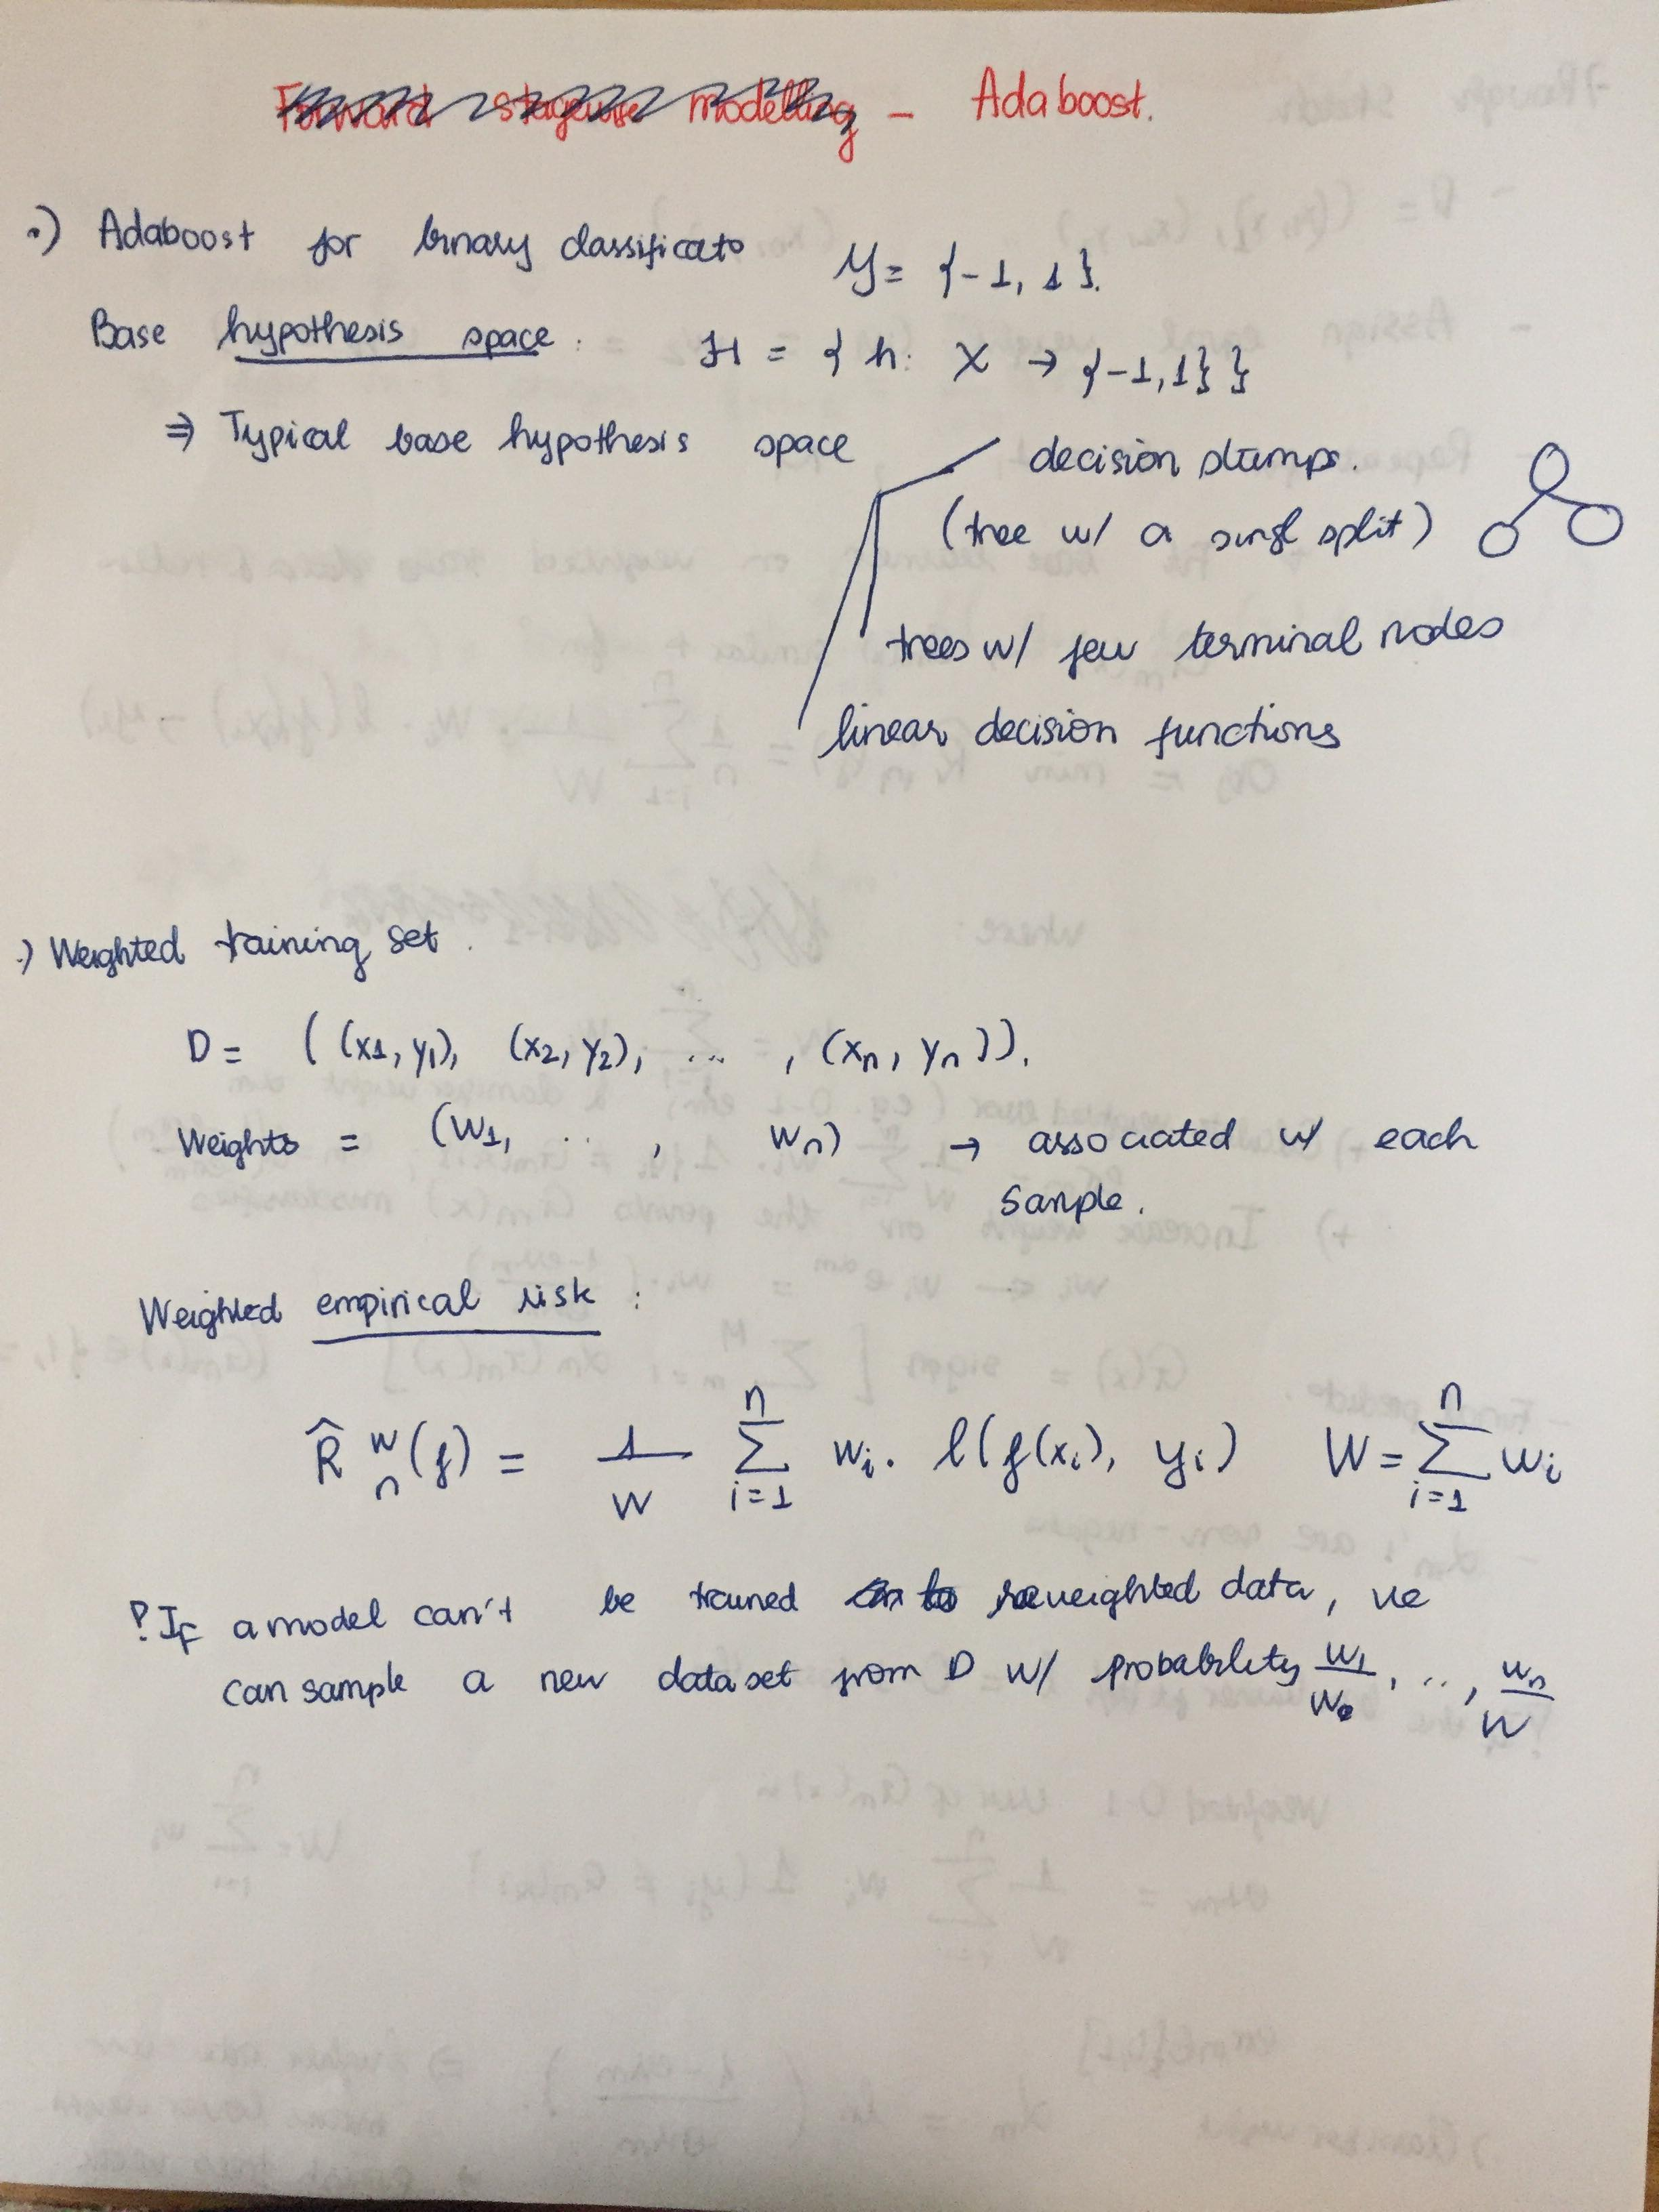
\includegraphics[max size={\textwidth}{0.9\textheight}]{Adaboost1.jpg} \\

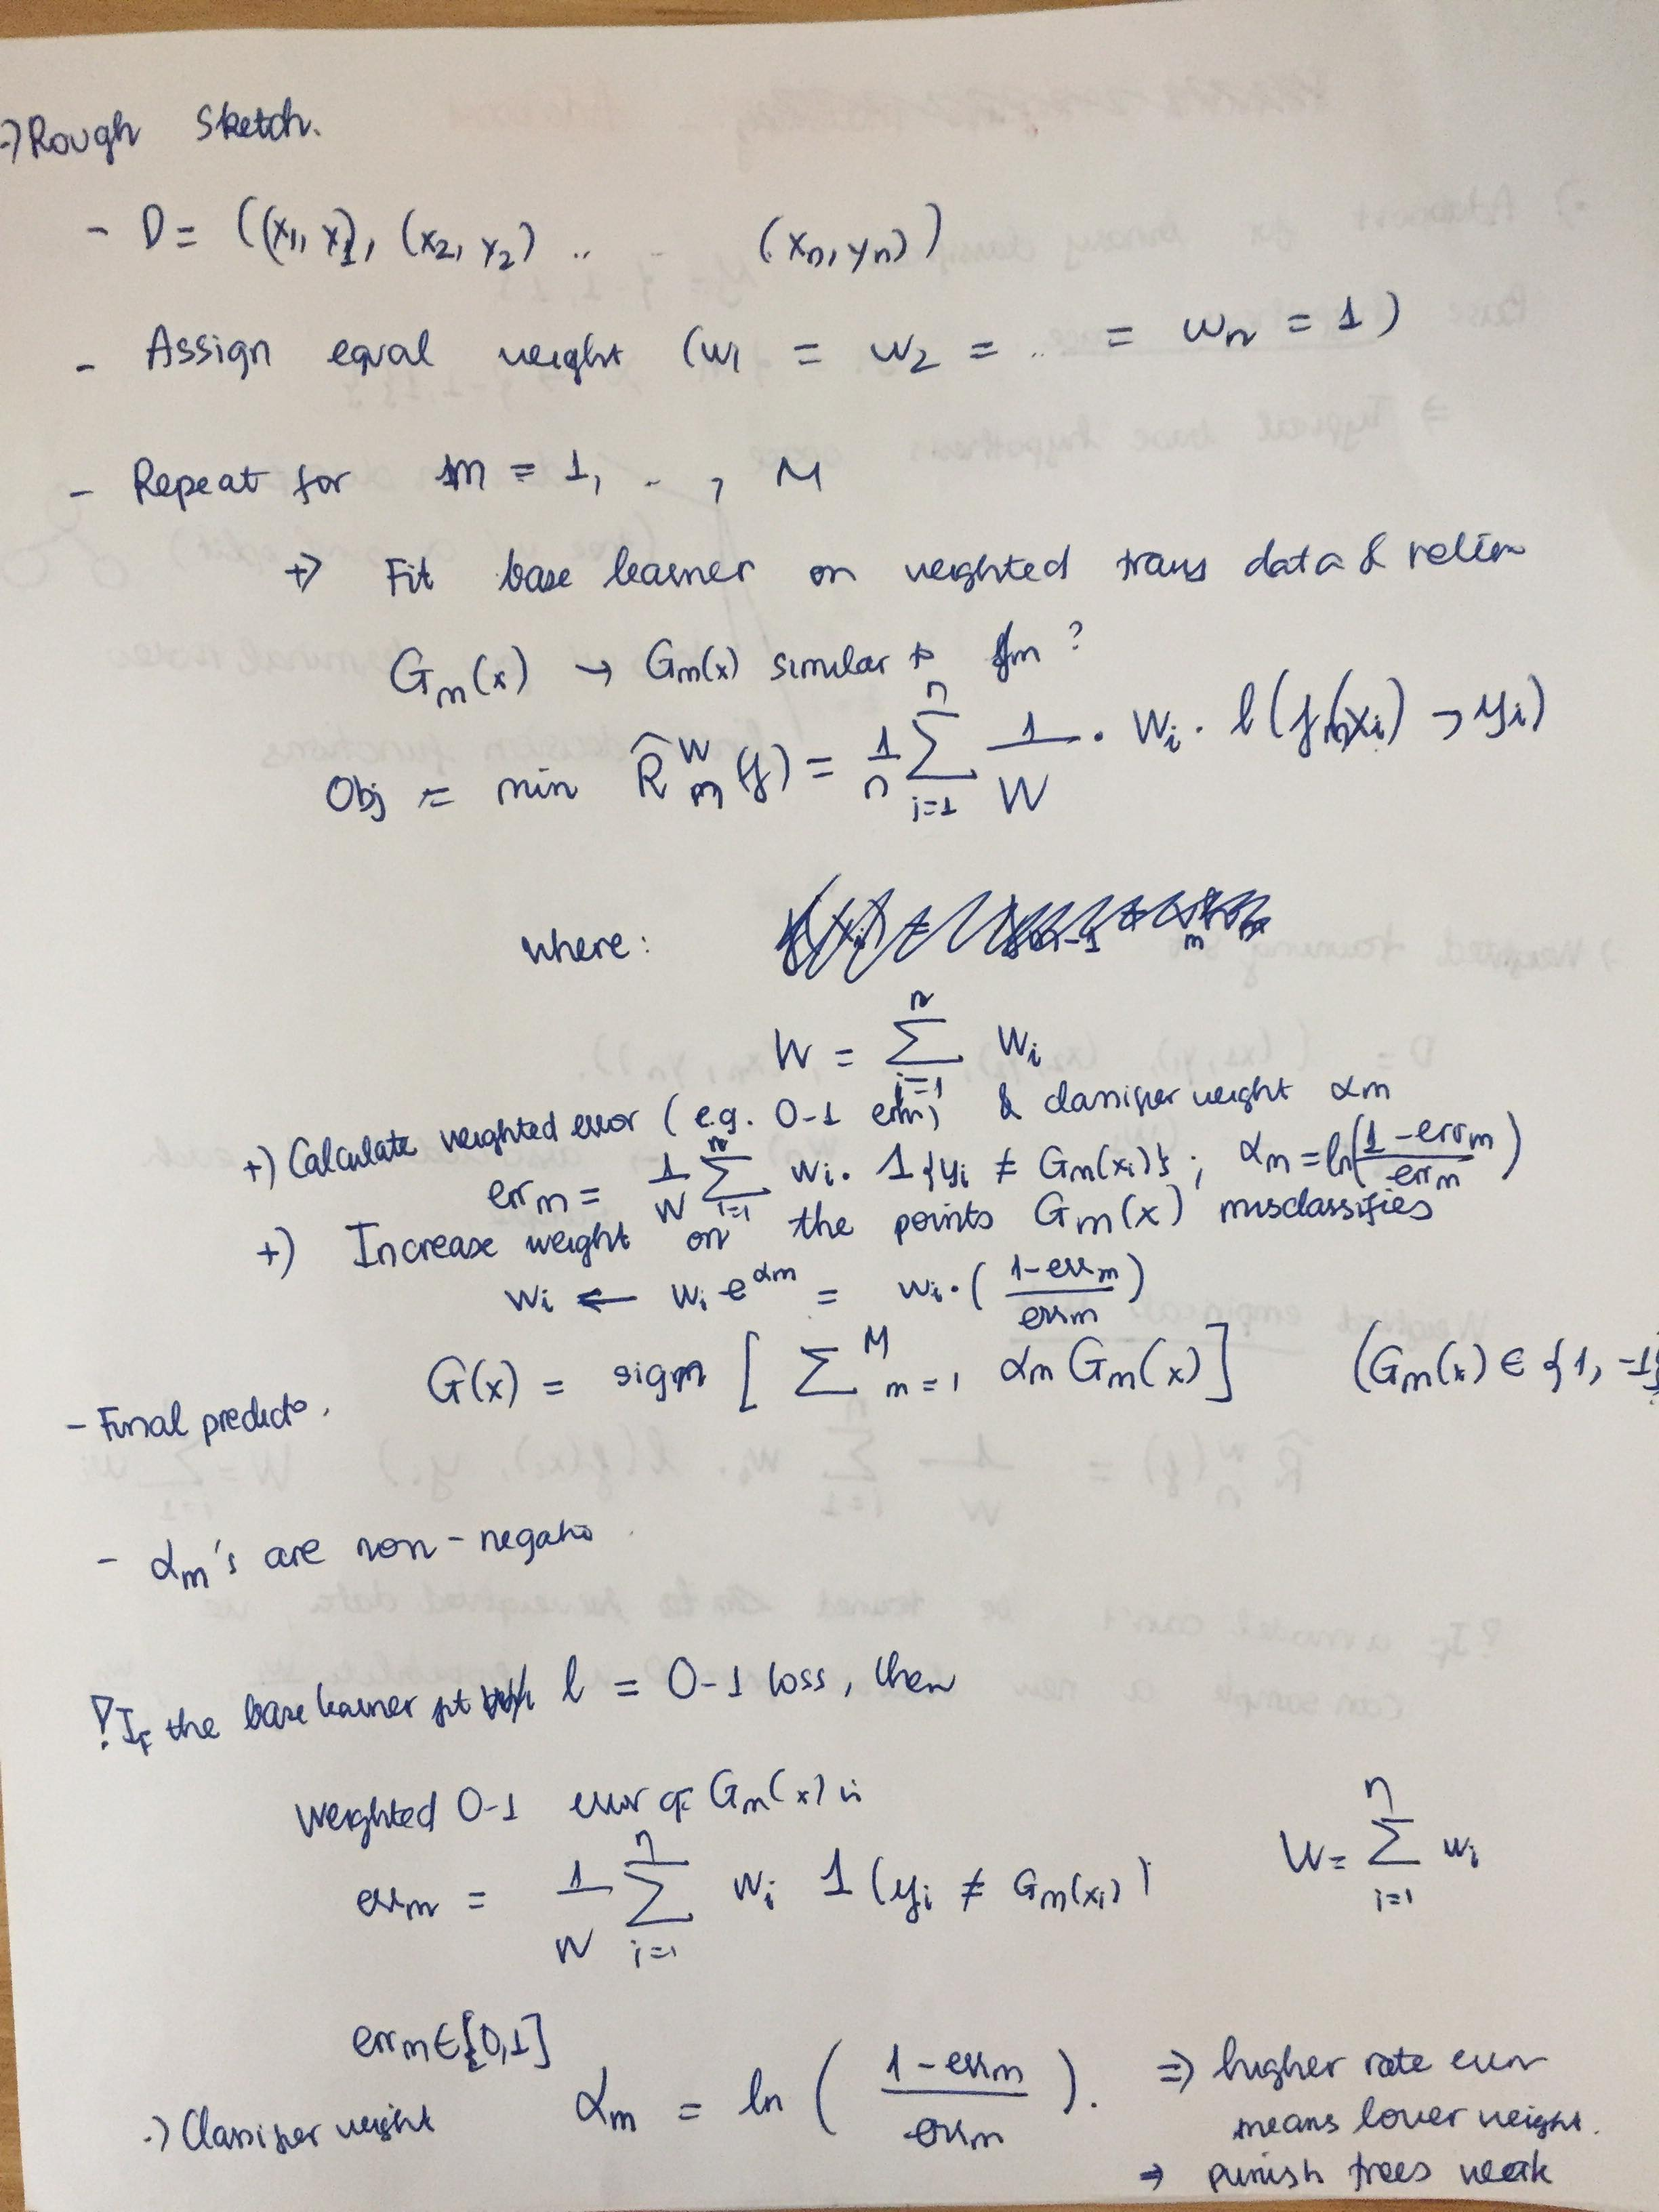
\includegraphics[max size={\textwidth}{\textheight}]{Adaboost2.jpg} 

\subsection{Forward Stage-wise Addictive Modeling }
 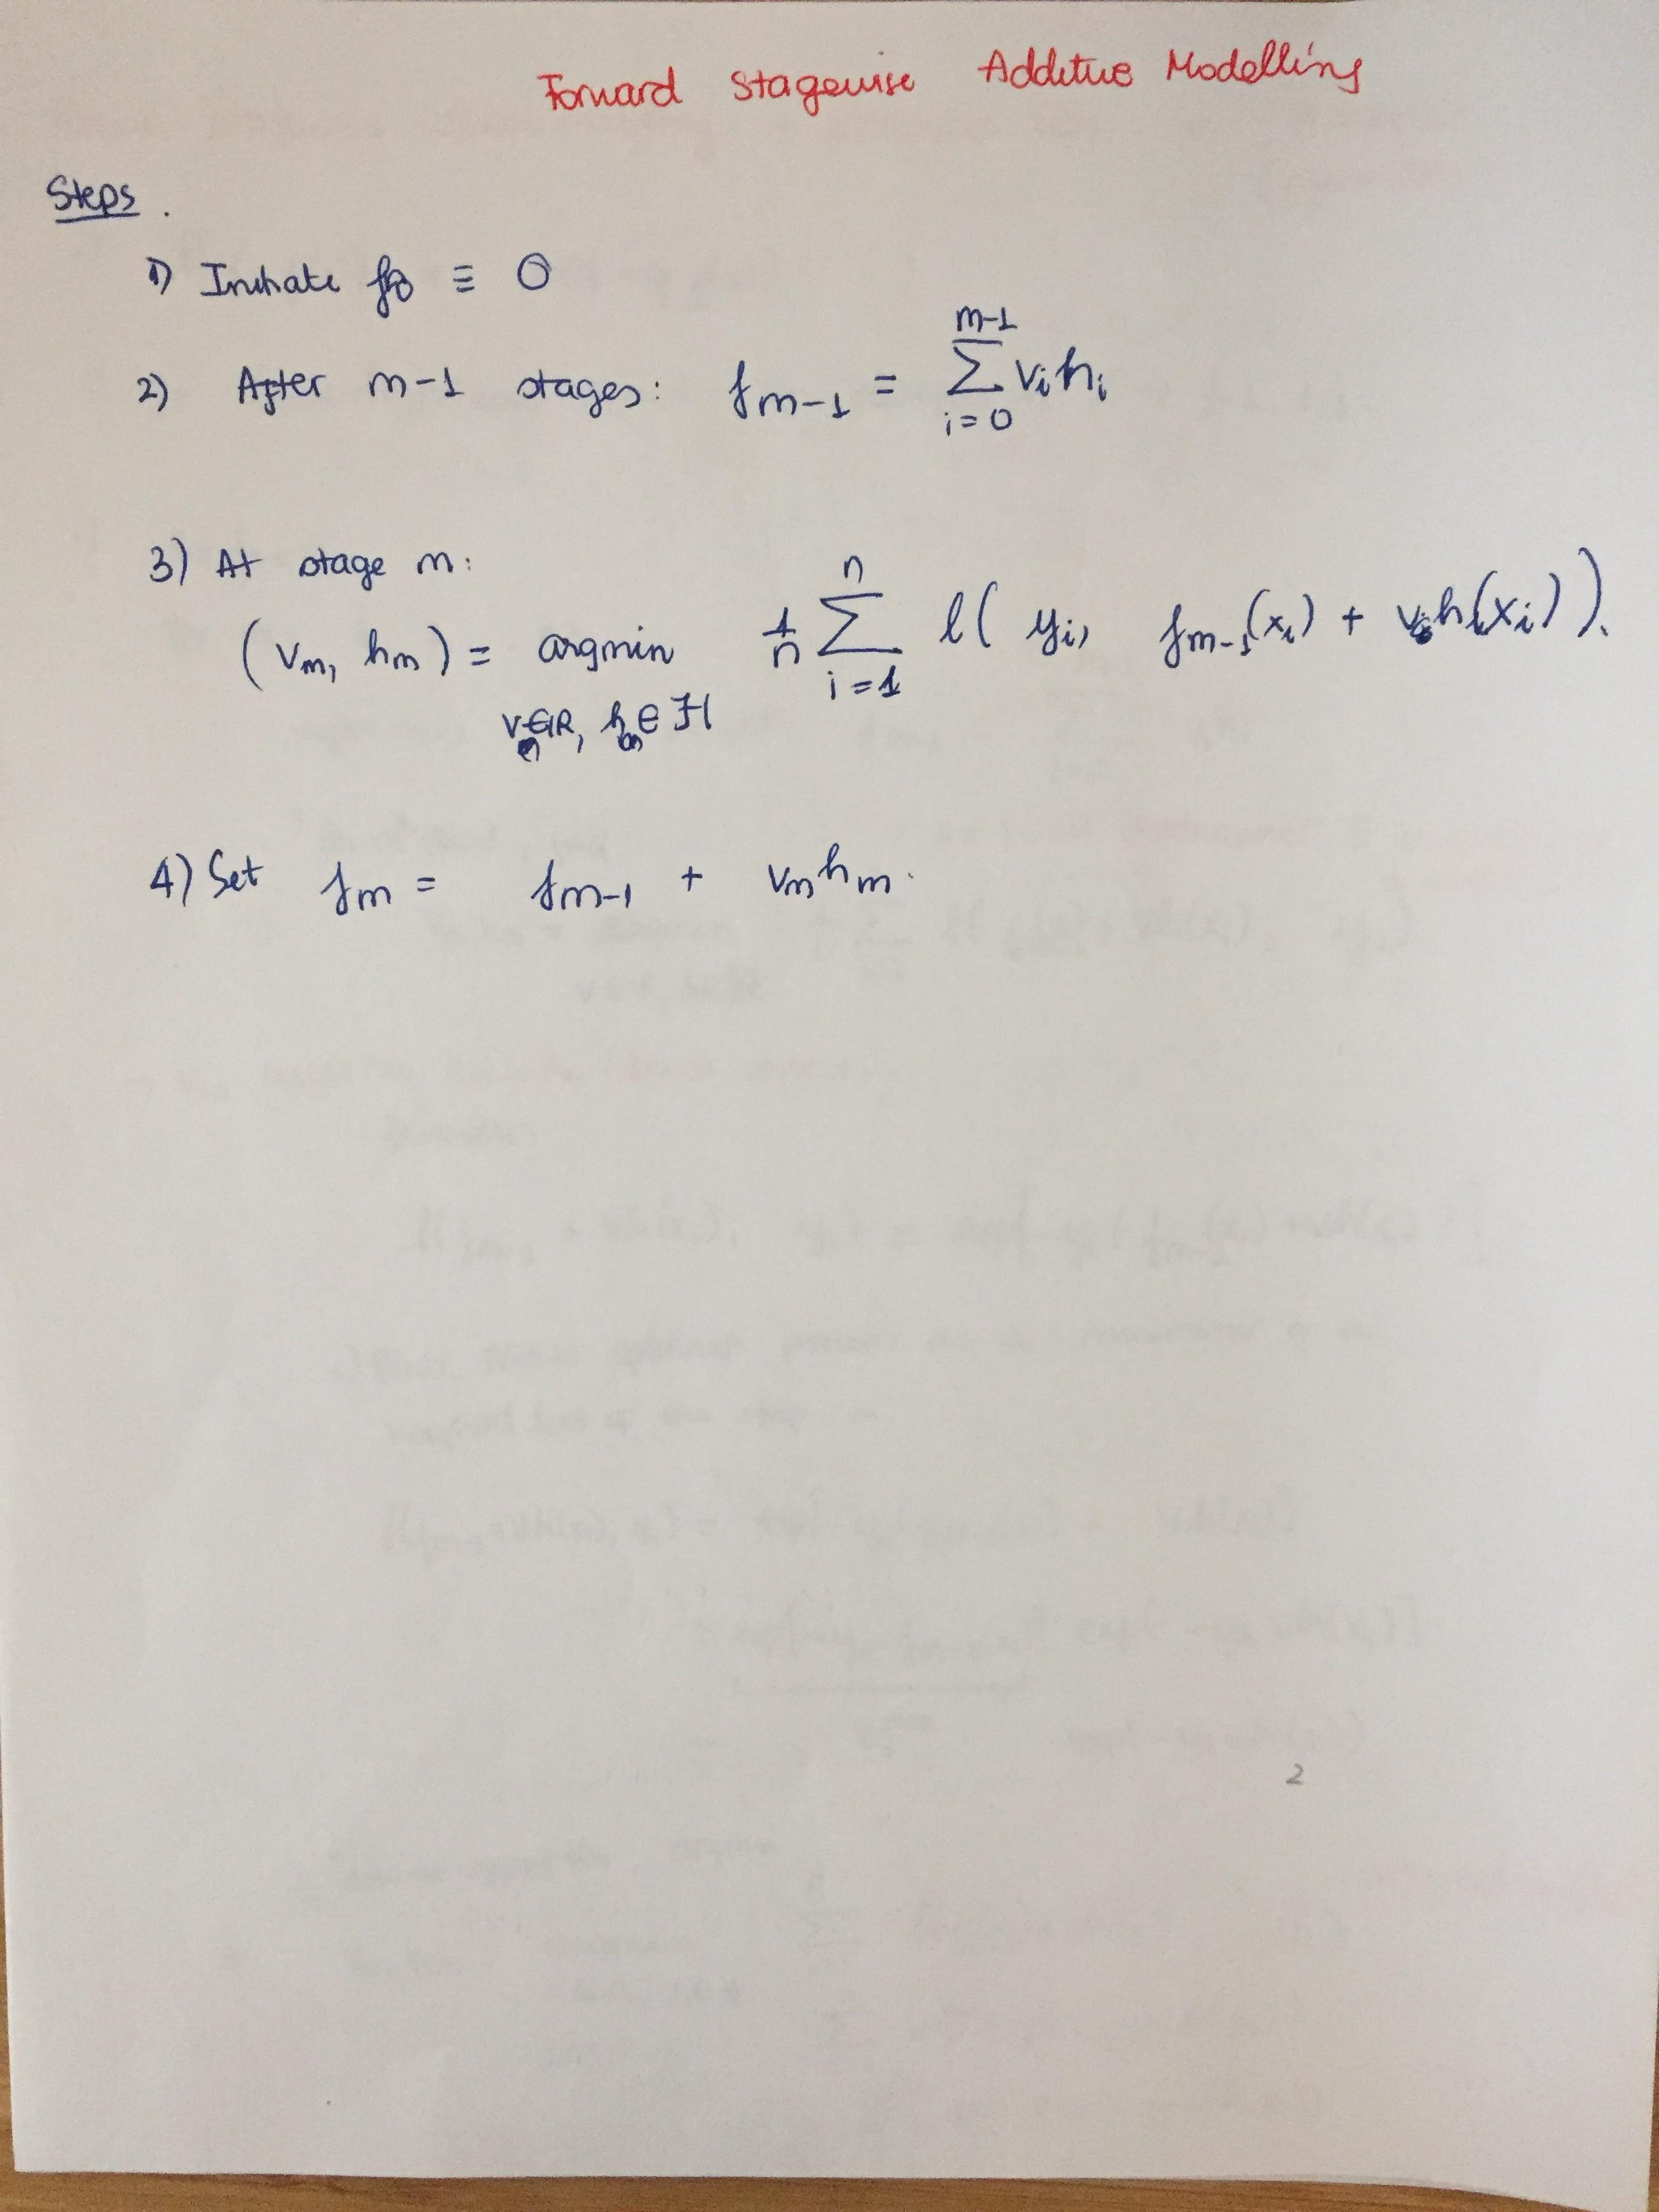
\includegraphics[max size={\textwidth}{0.9\textheight}]{FSAM1.jpg} \\
 
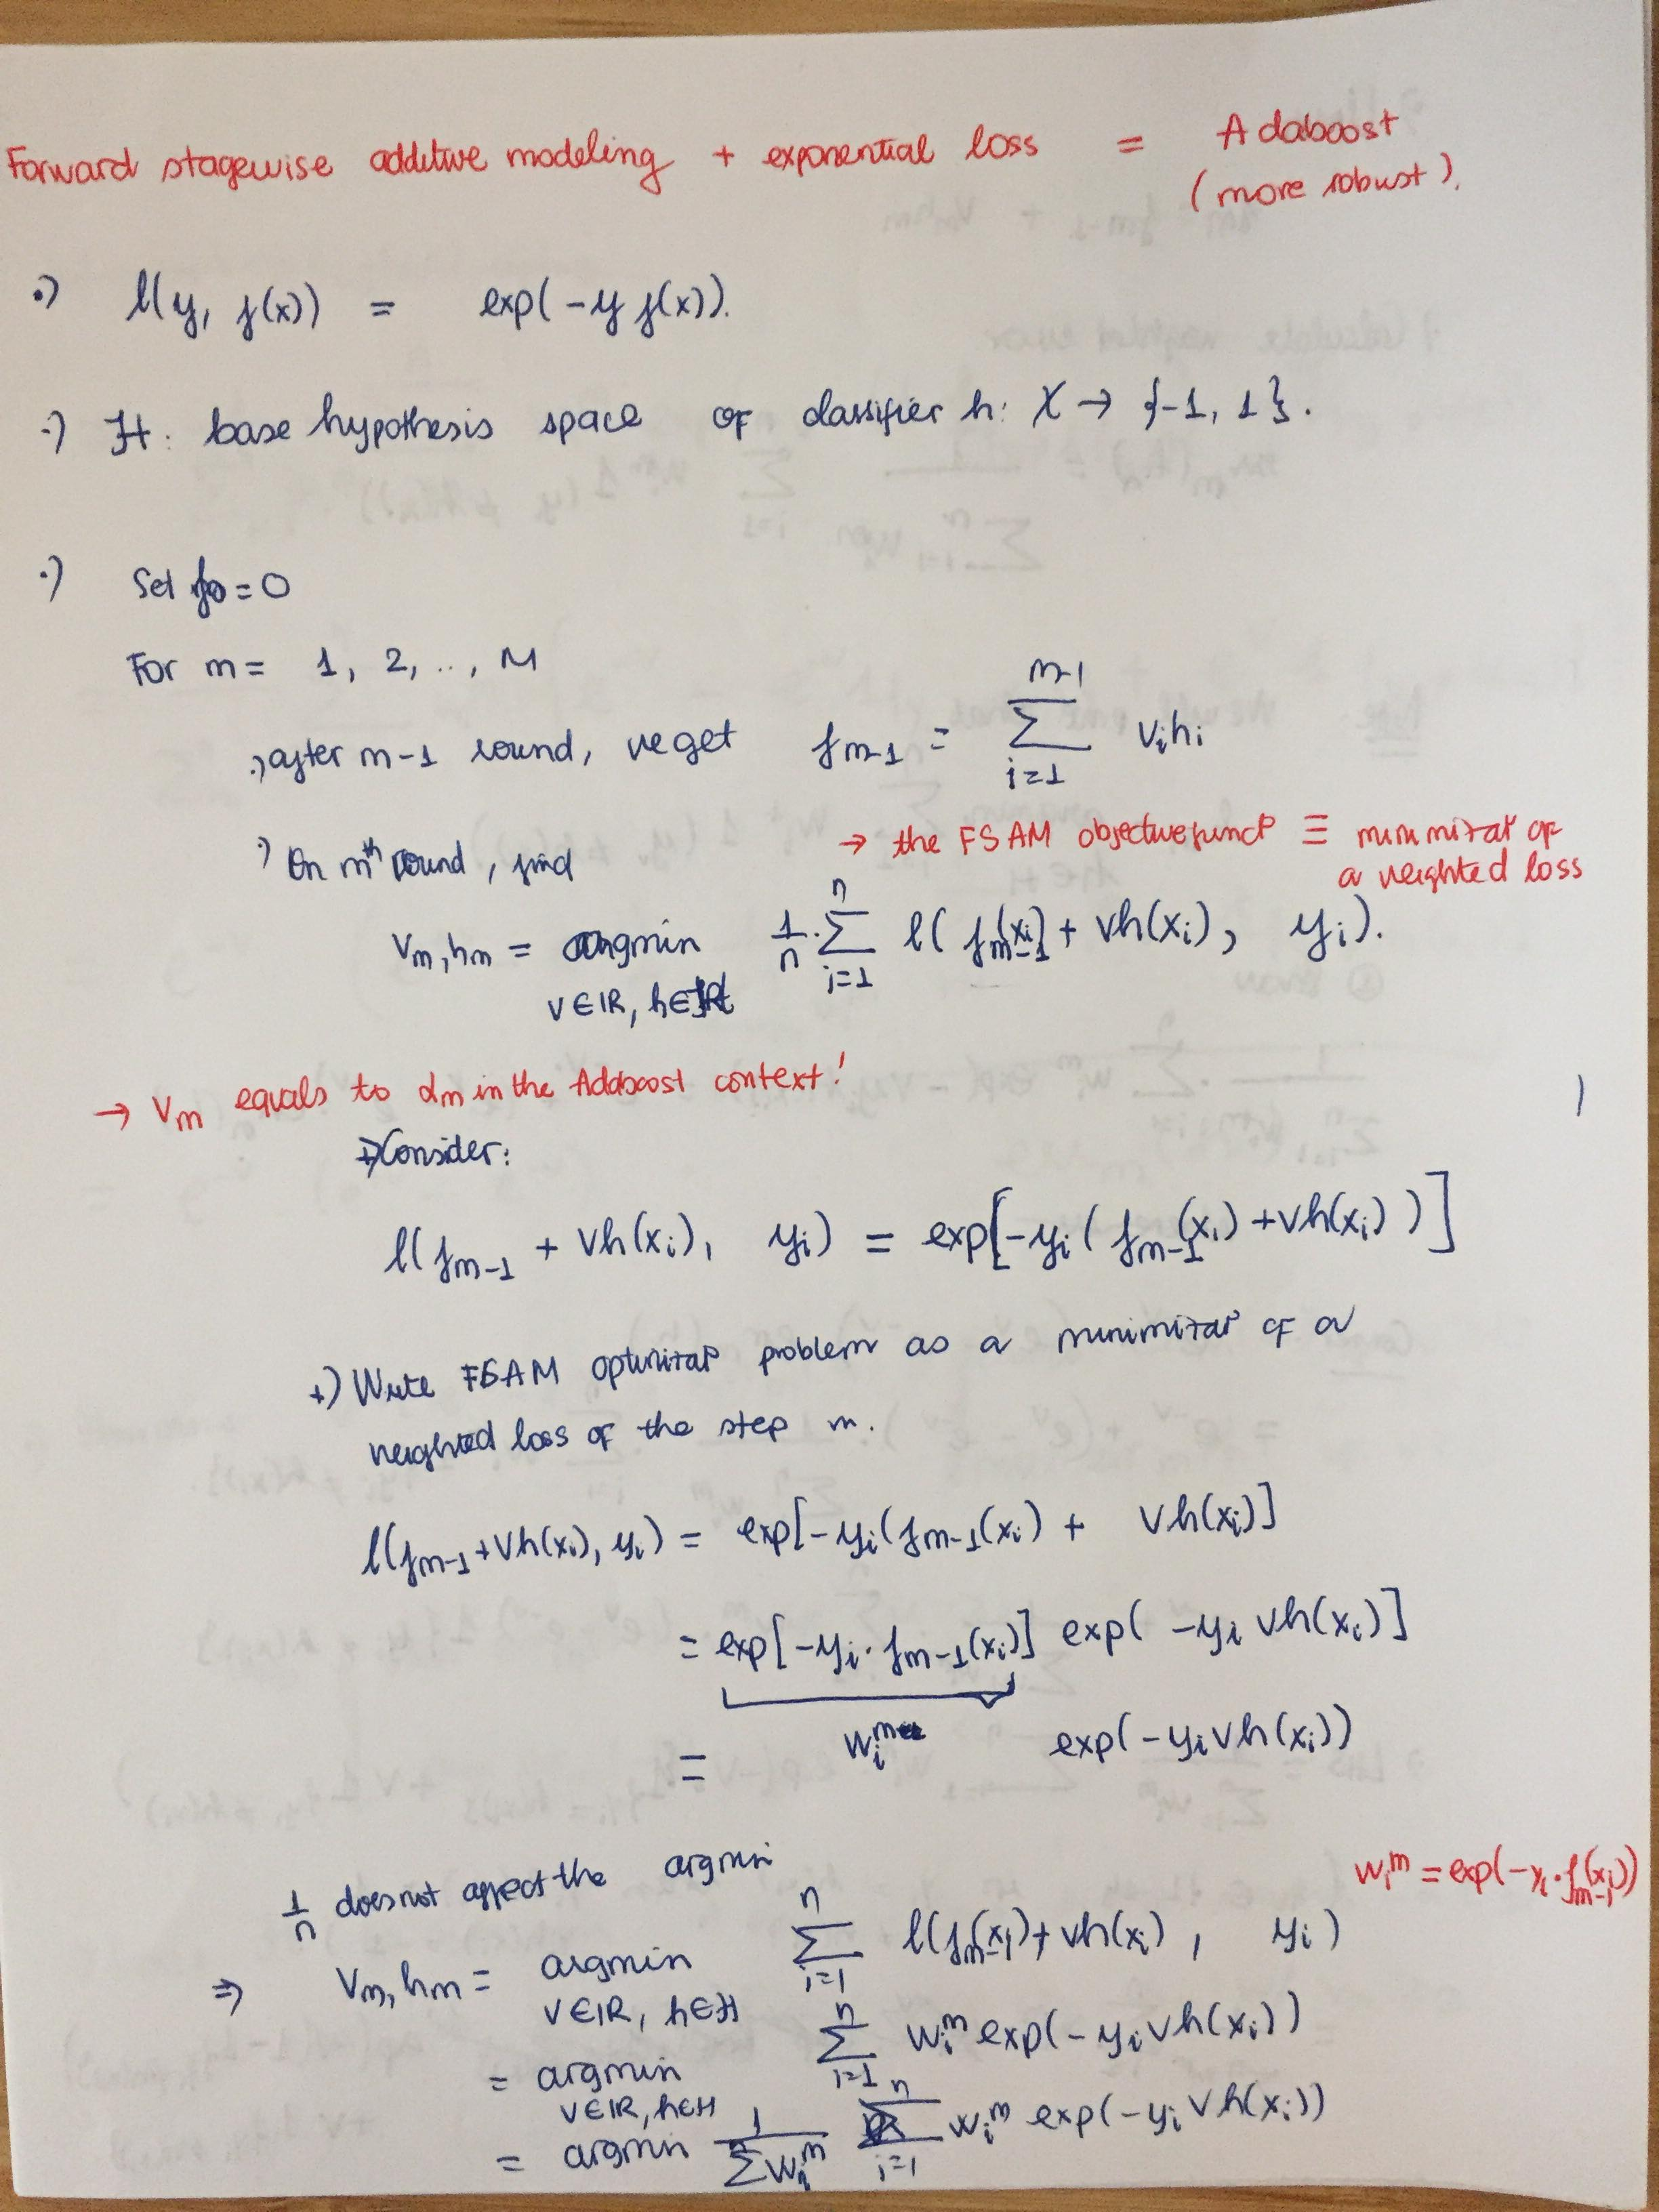
\includegraphics[max size={\textwidth}{0.9\textheight}]{FSAM2.jpg} \\
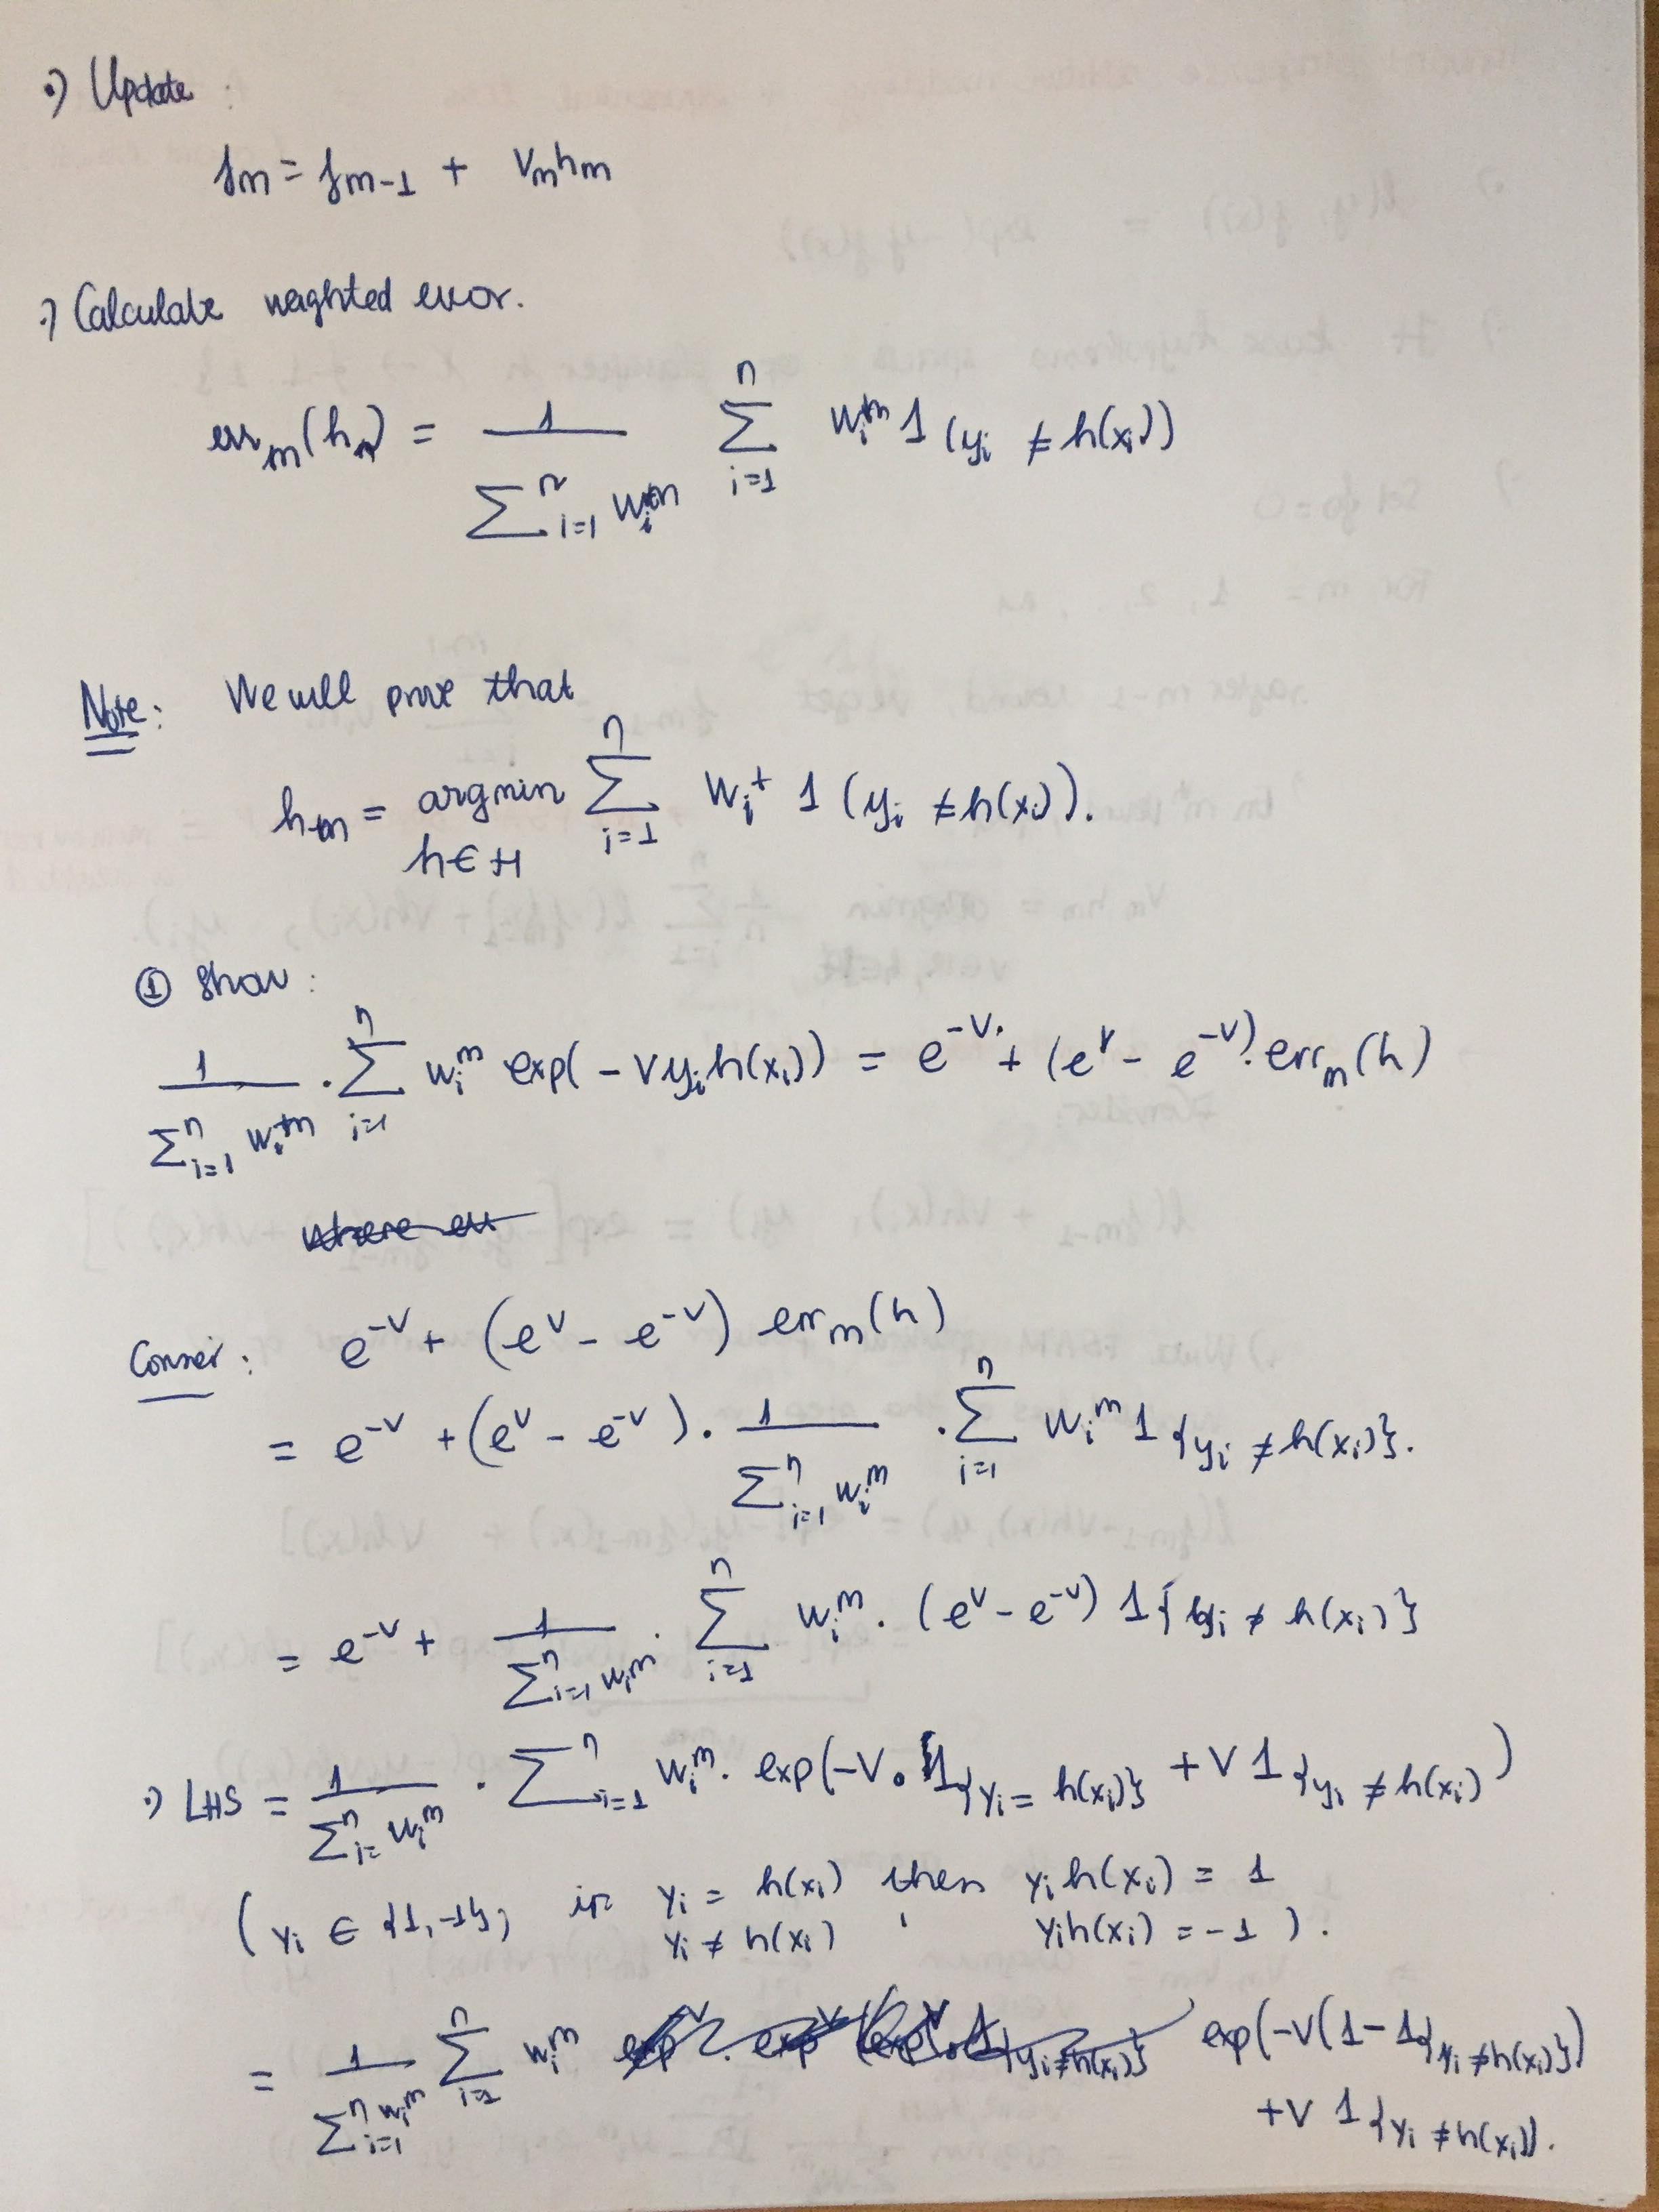
\includegraphics[max size={\textwidth}{0.9\textheight}]{FSAM3.jpg} \\
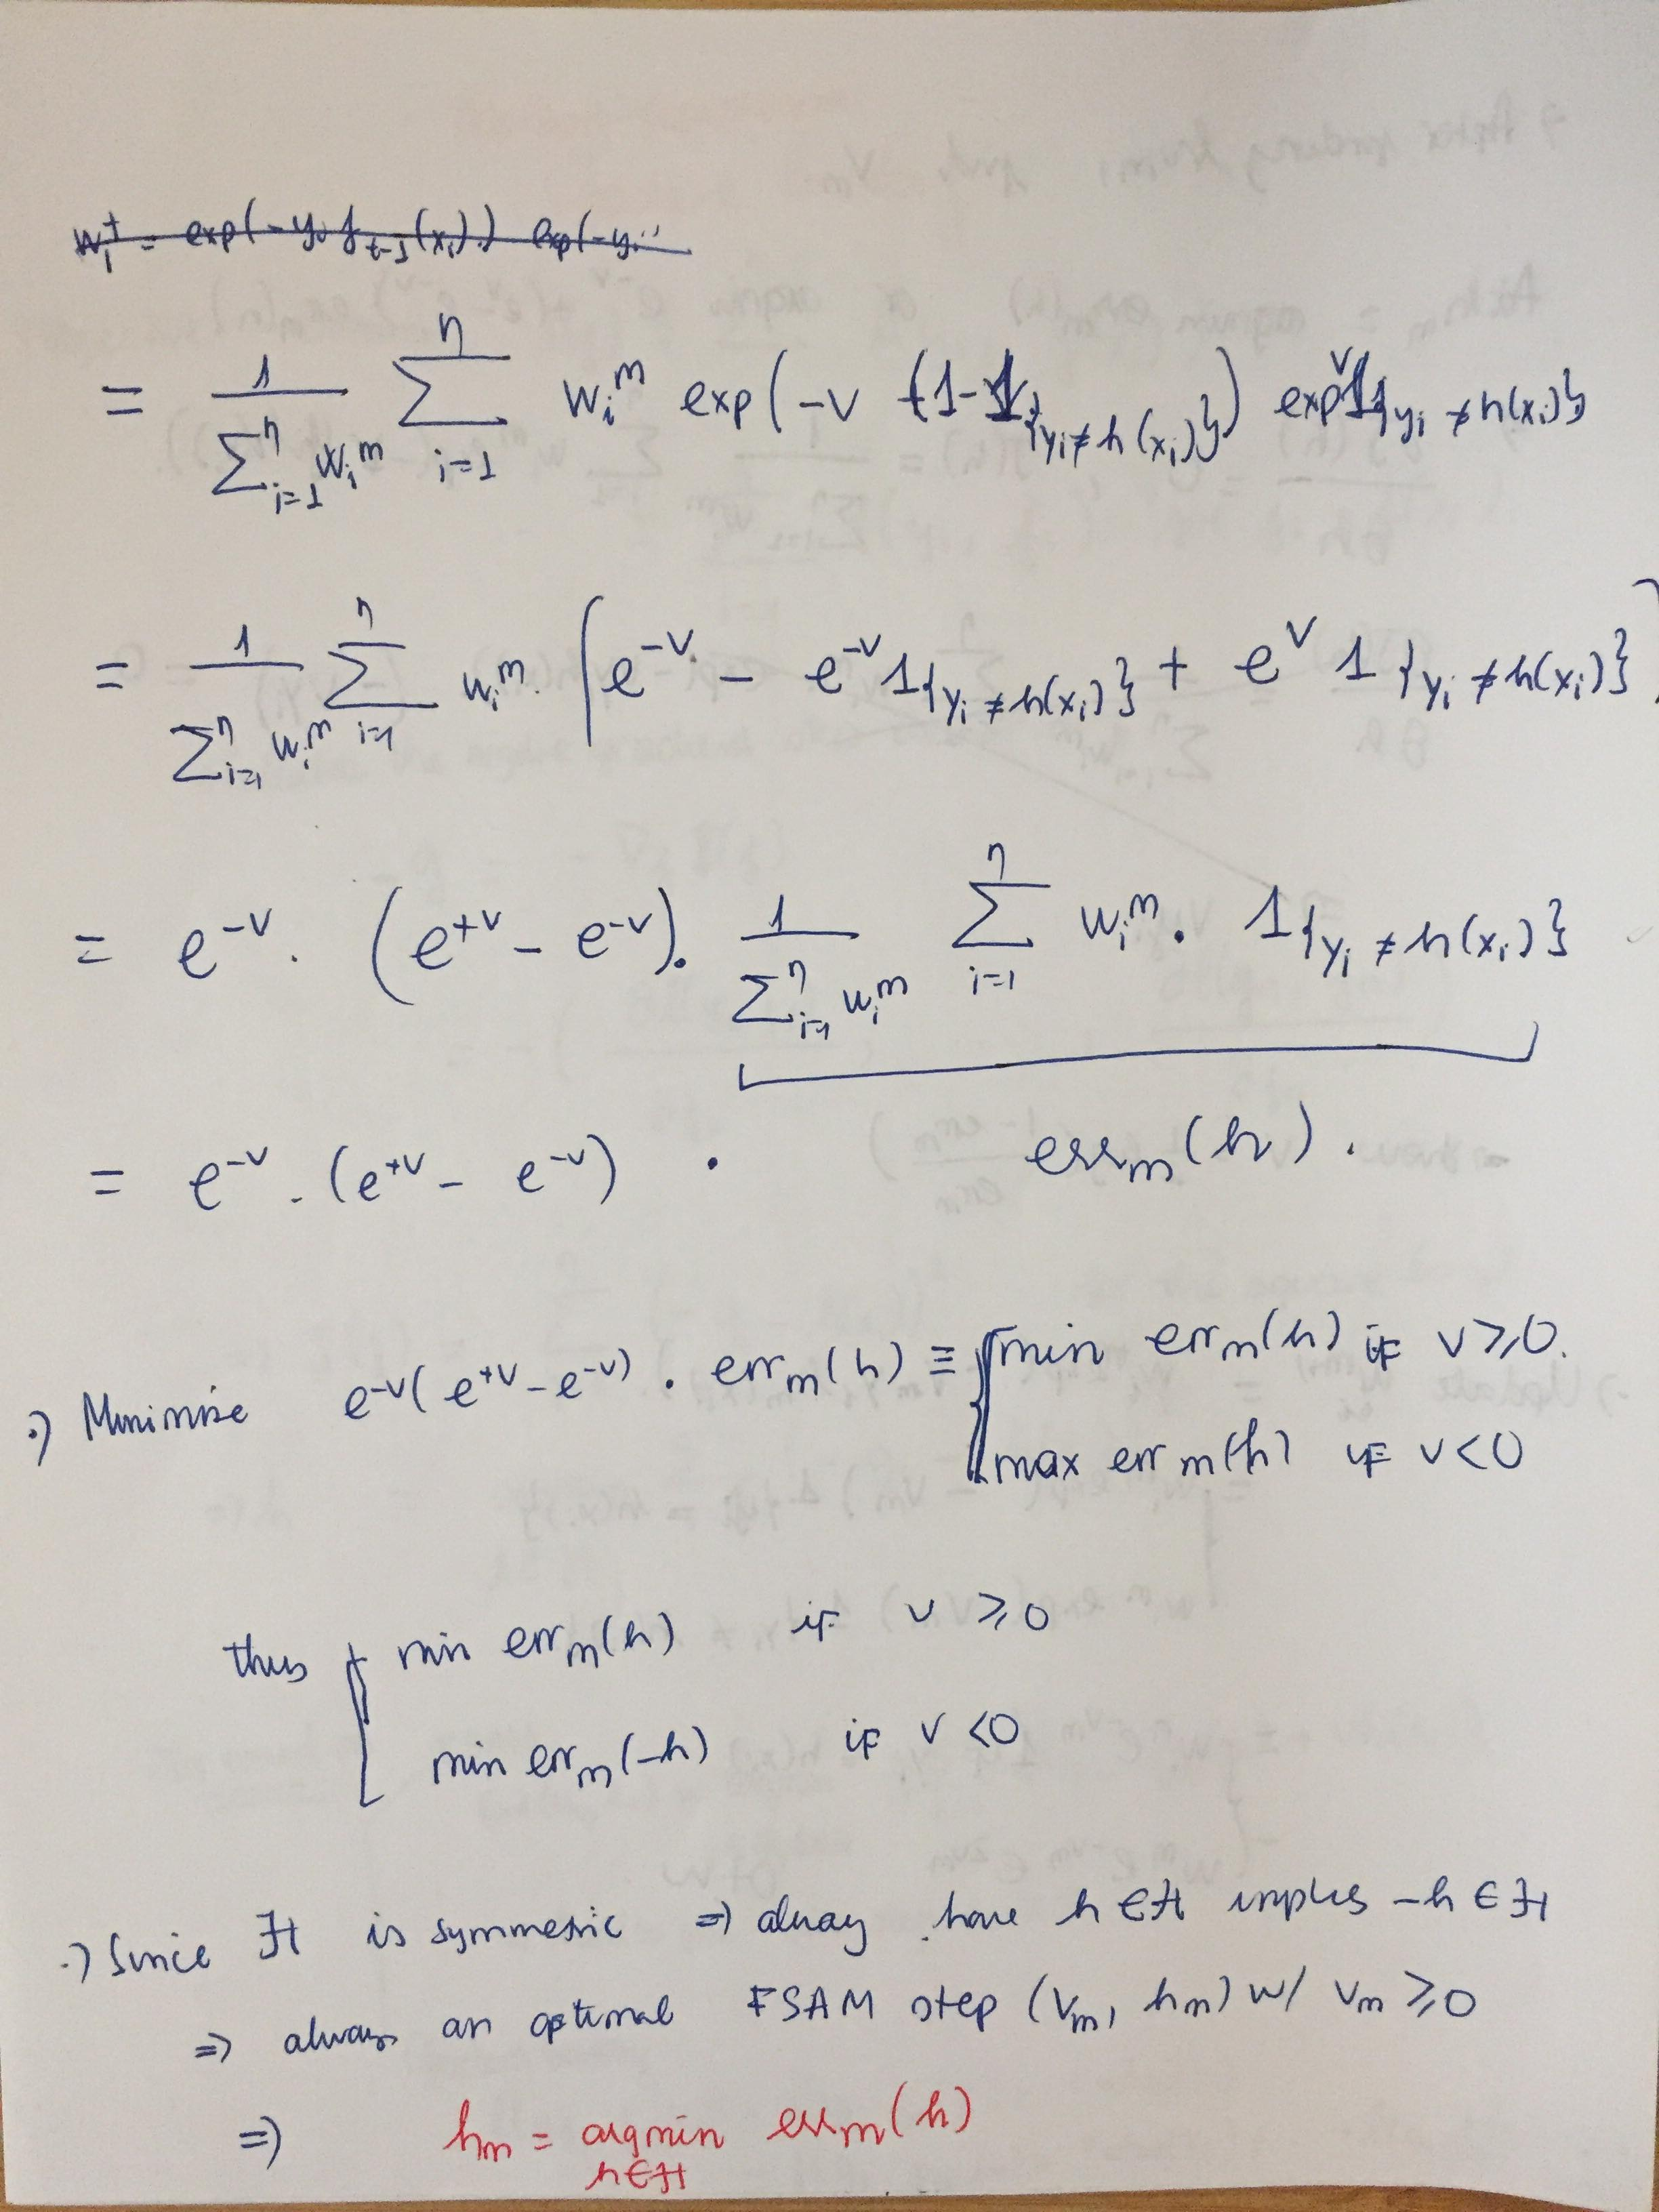
\includegraphics[max size={\textwidth}{0.9\textheight}]{FSAM4.jpg} \\
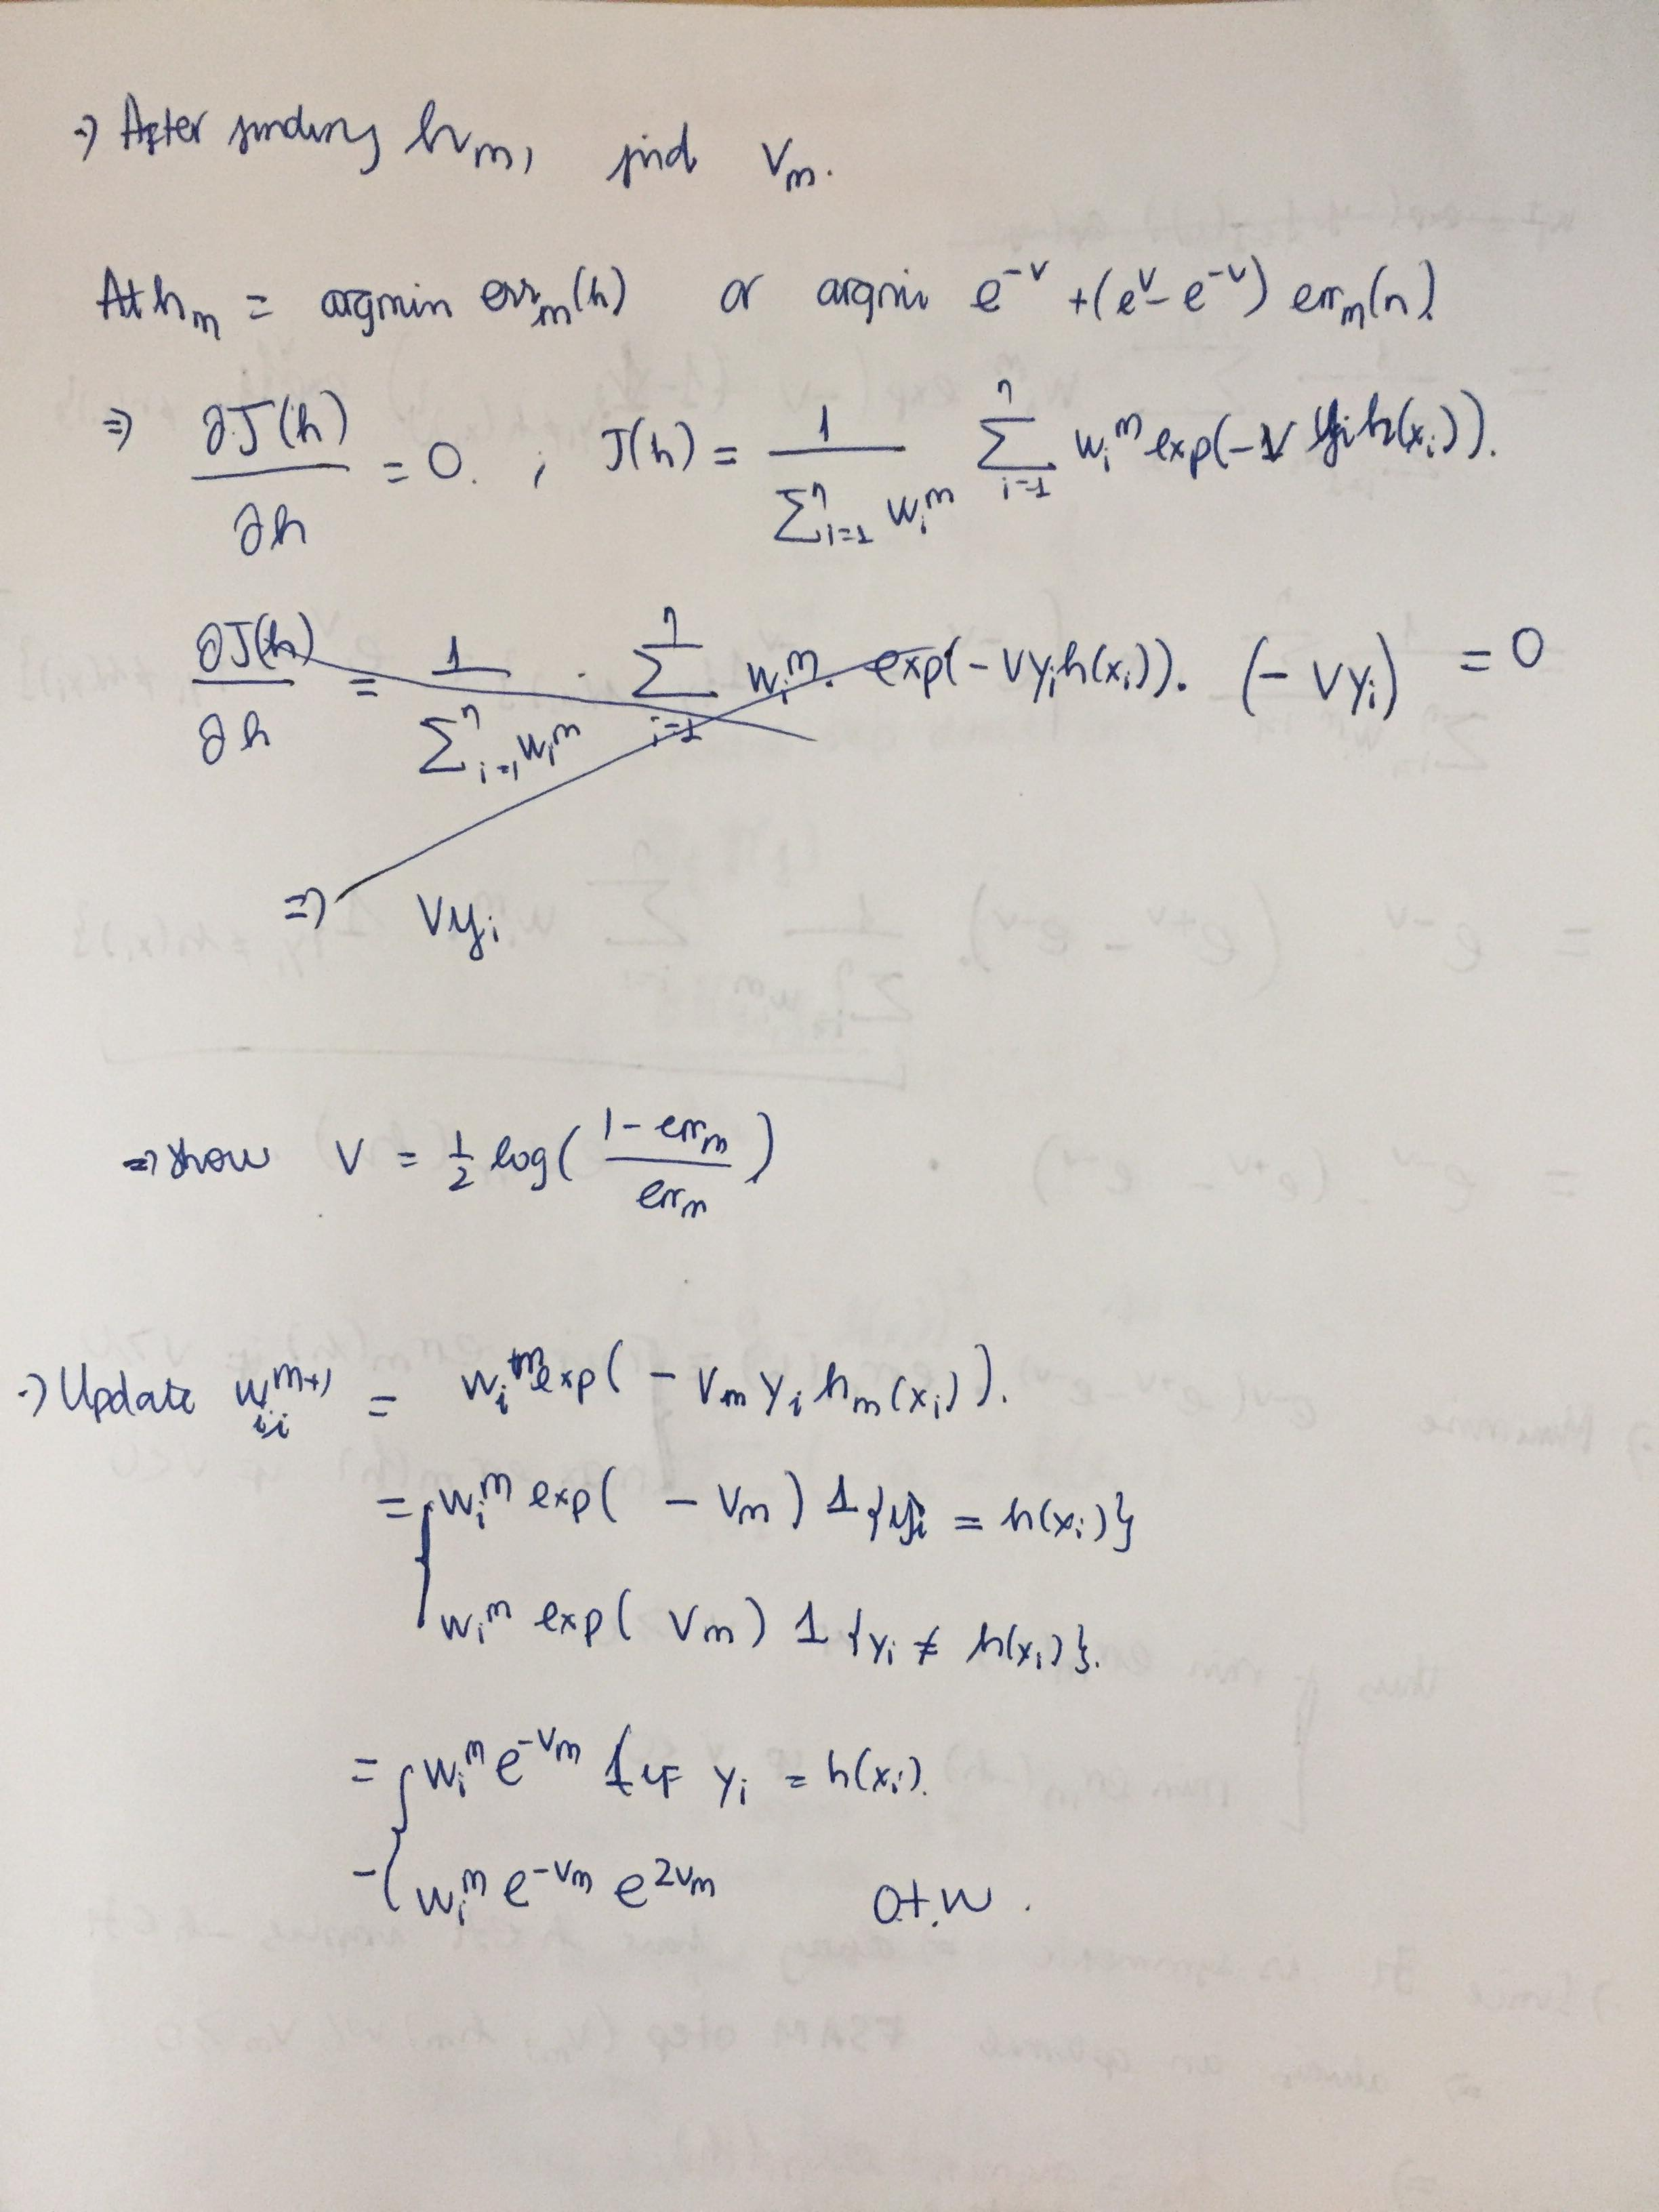
\includegraphics[max size={\textwidth}{0.9\textheight}]{FSAM5.jpg} 

\subsection{Gradient Bossting }
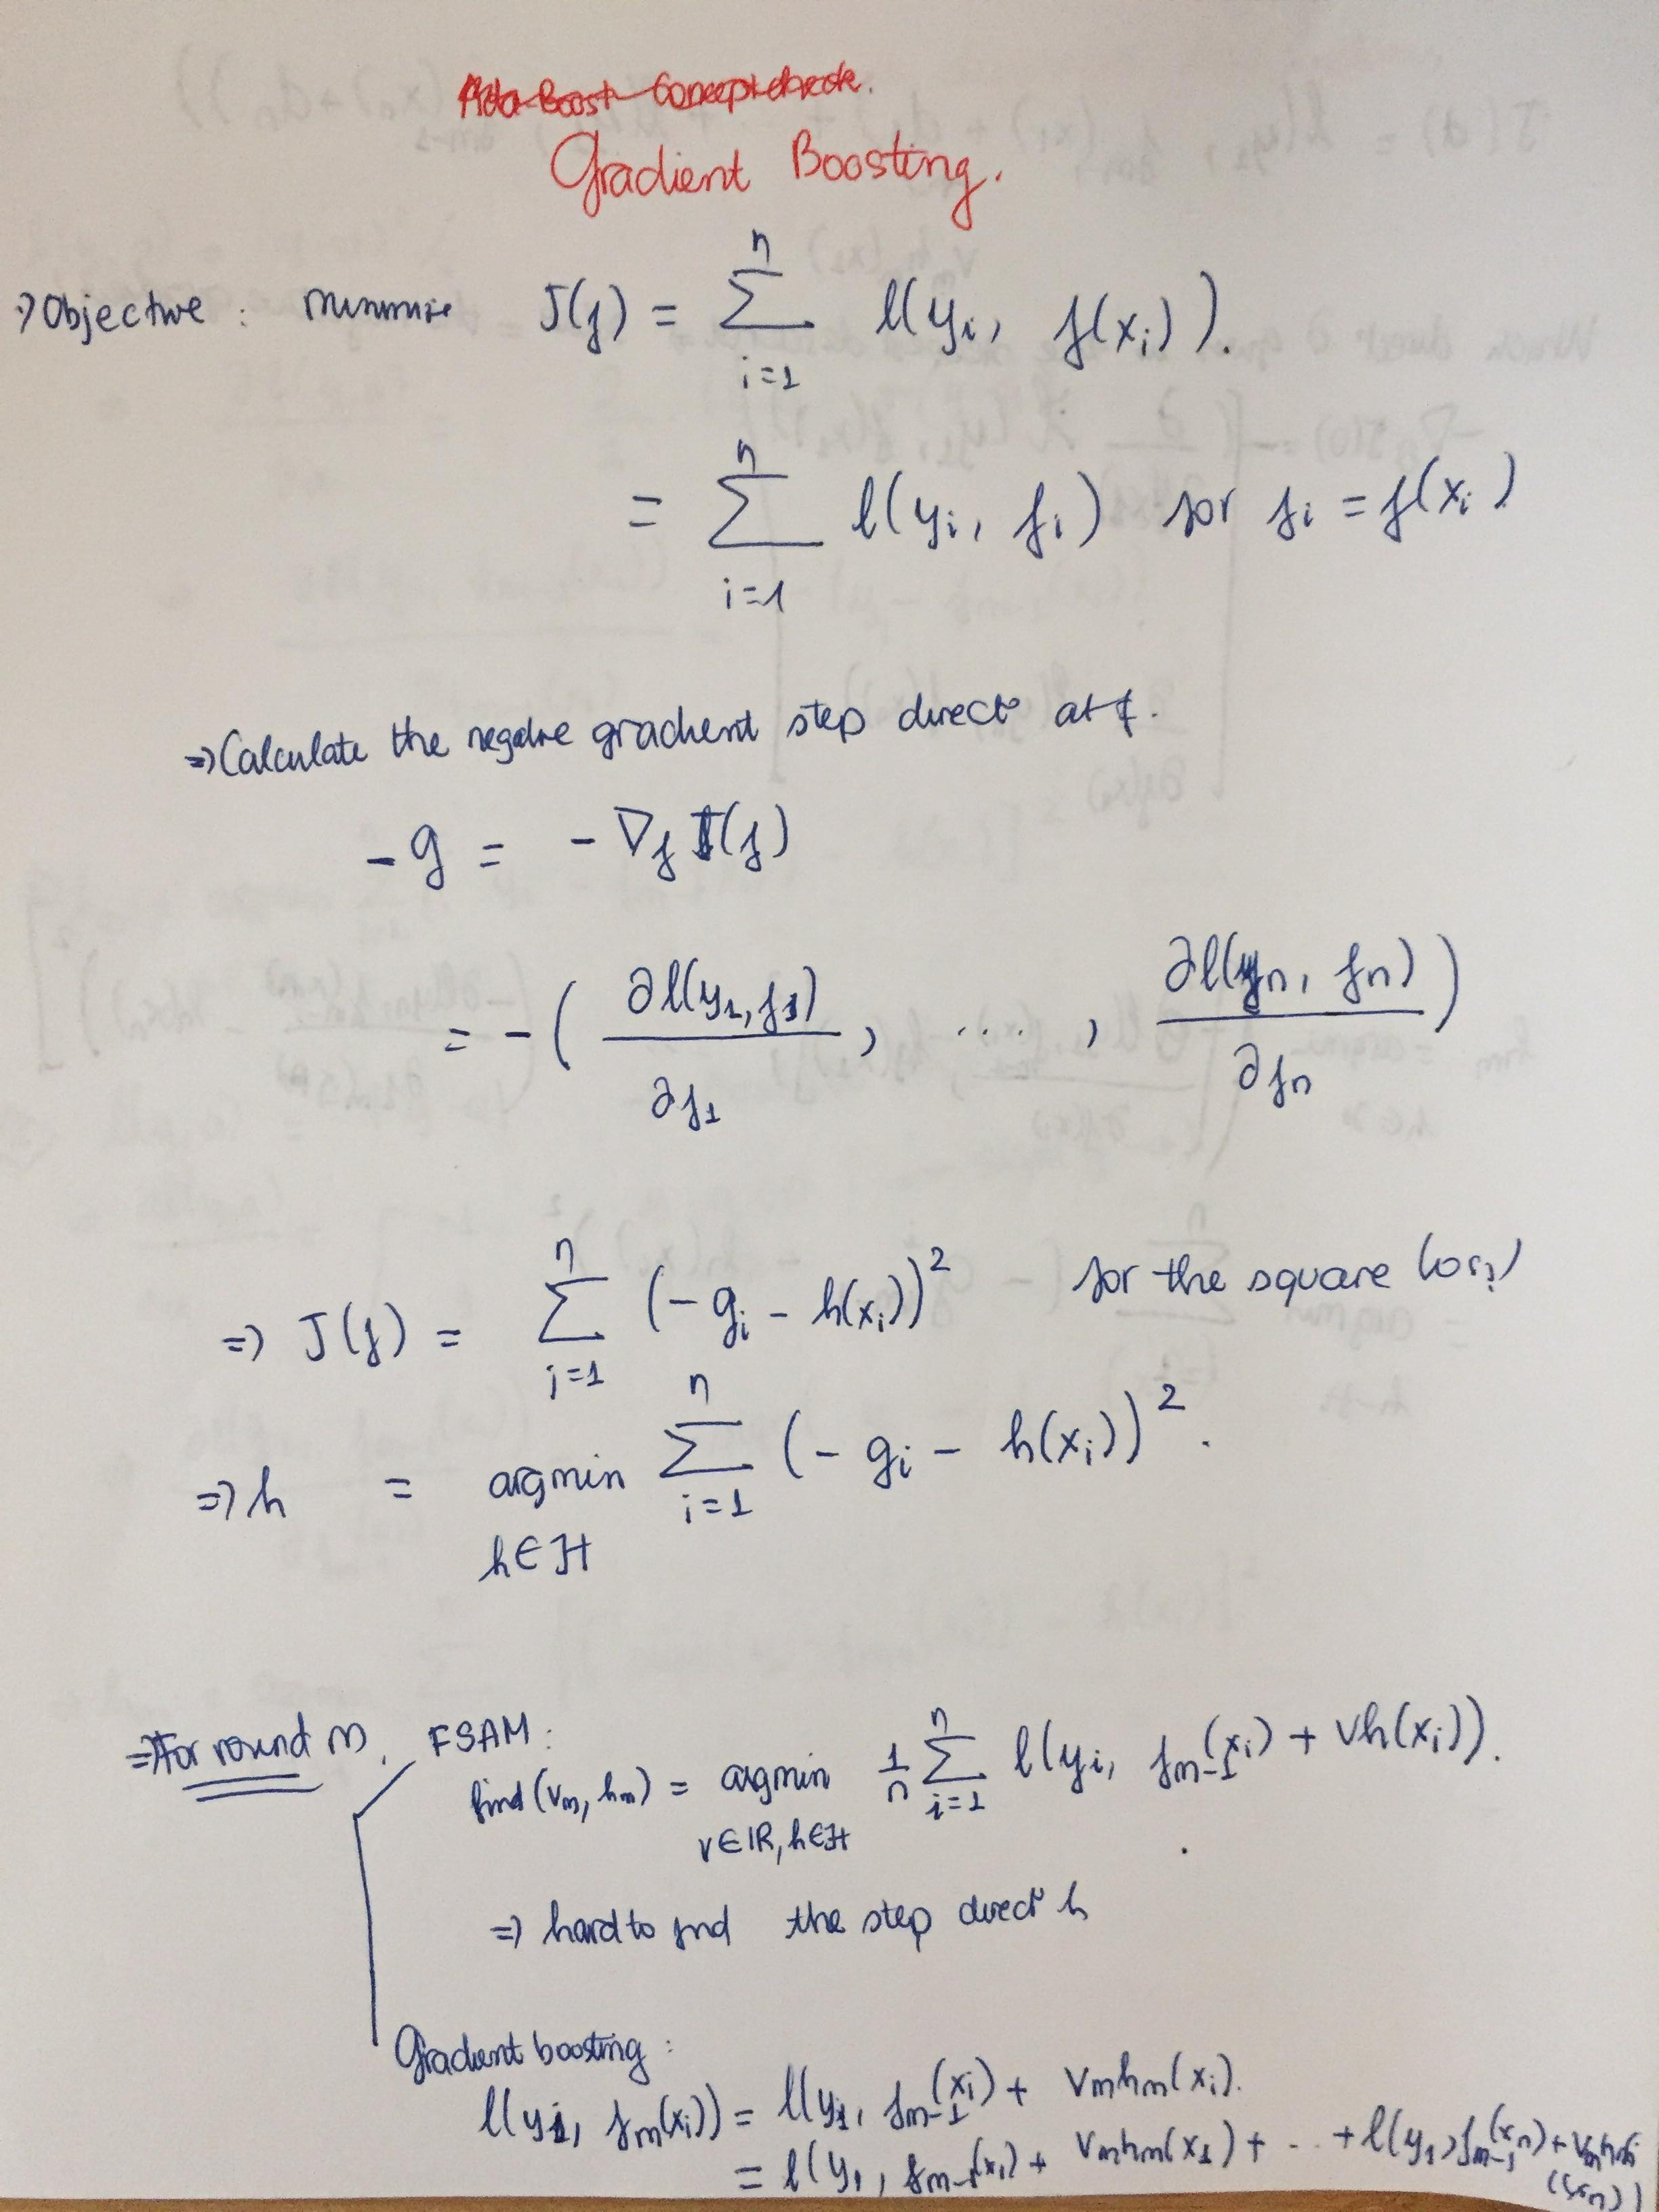
\includegraphics[max size={\textwidth}{0.9\textheight}]{GBM1.jpg}\\ 

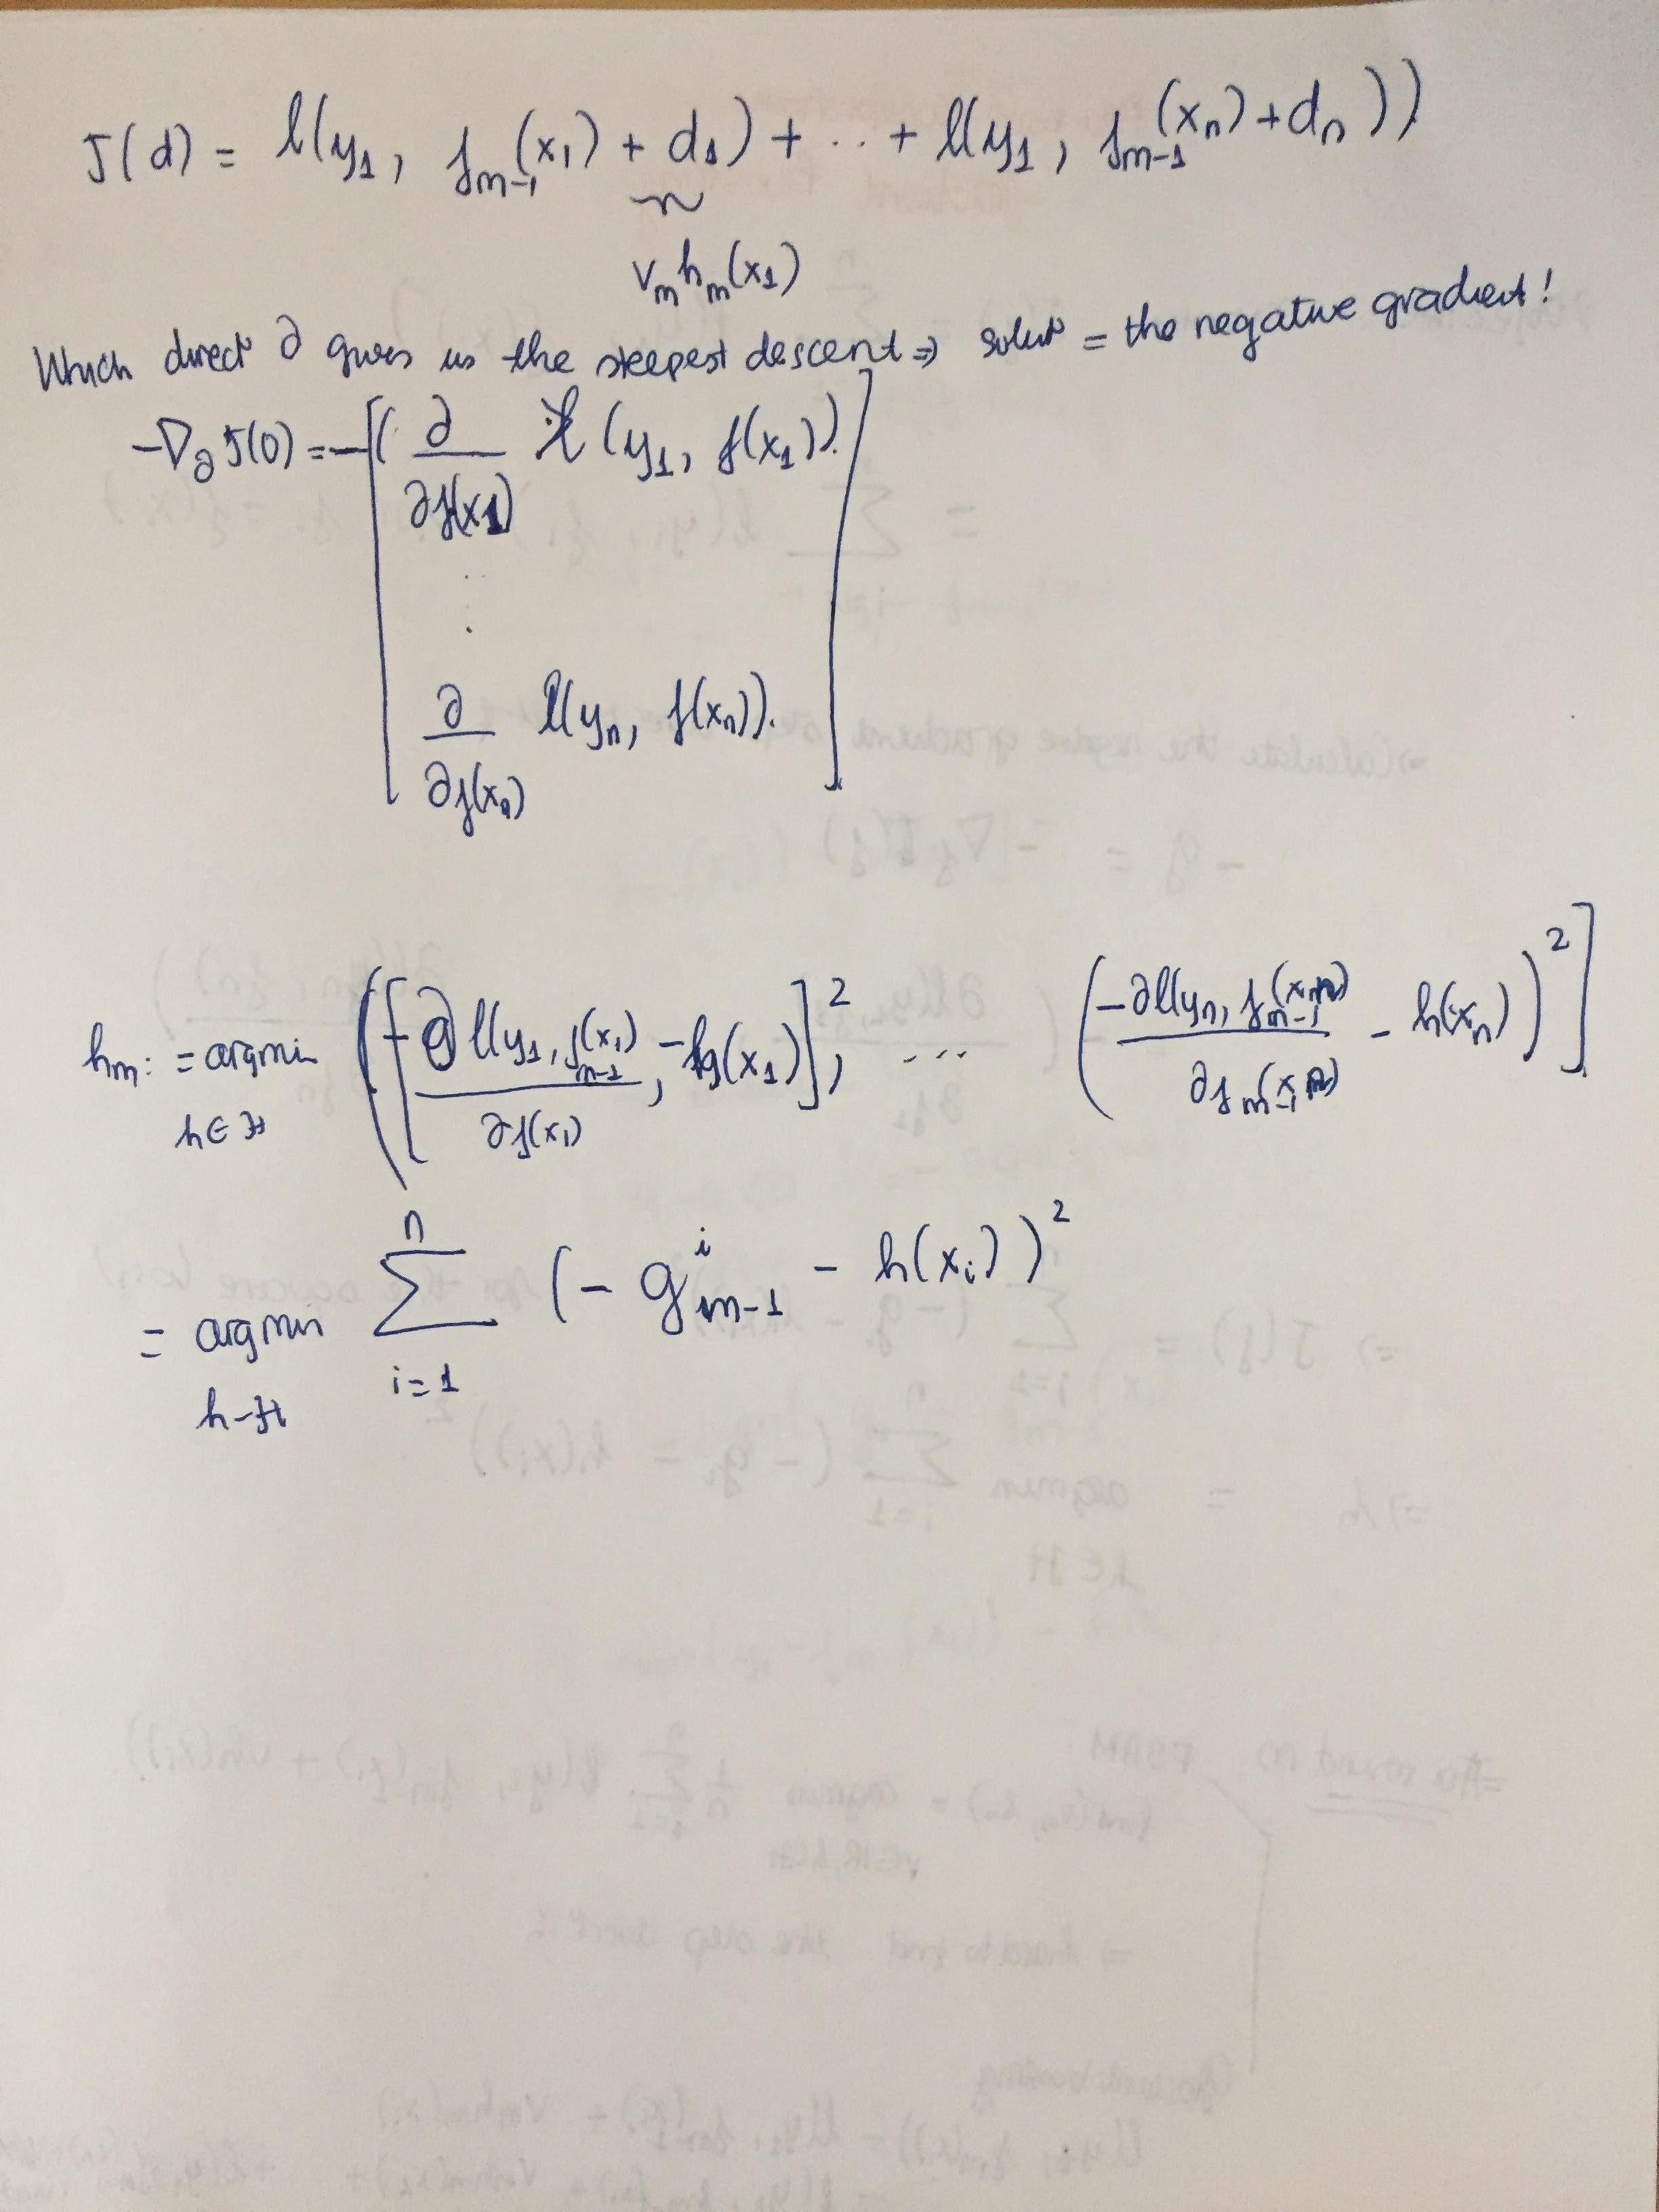
\includegraphics[max size={\textwidth}{0.9\textheight}]{GBM2.jpg} \\

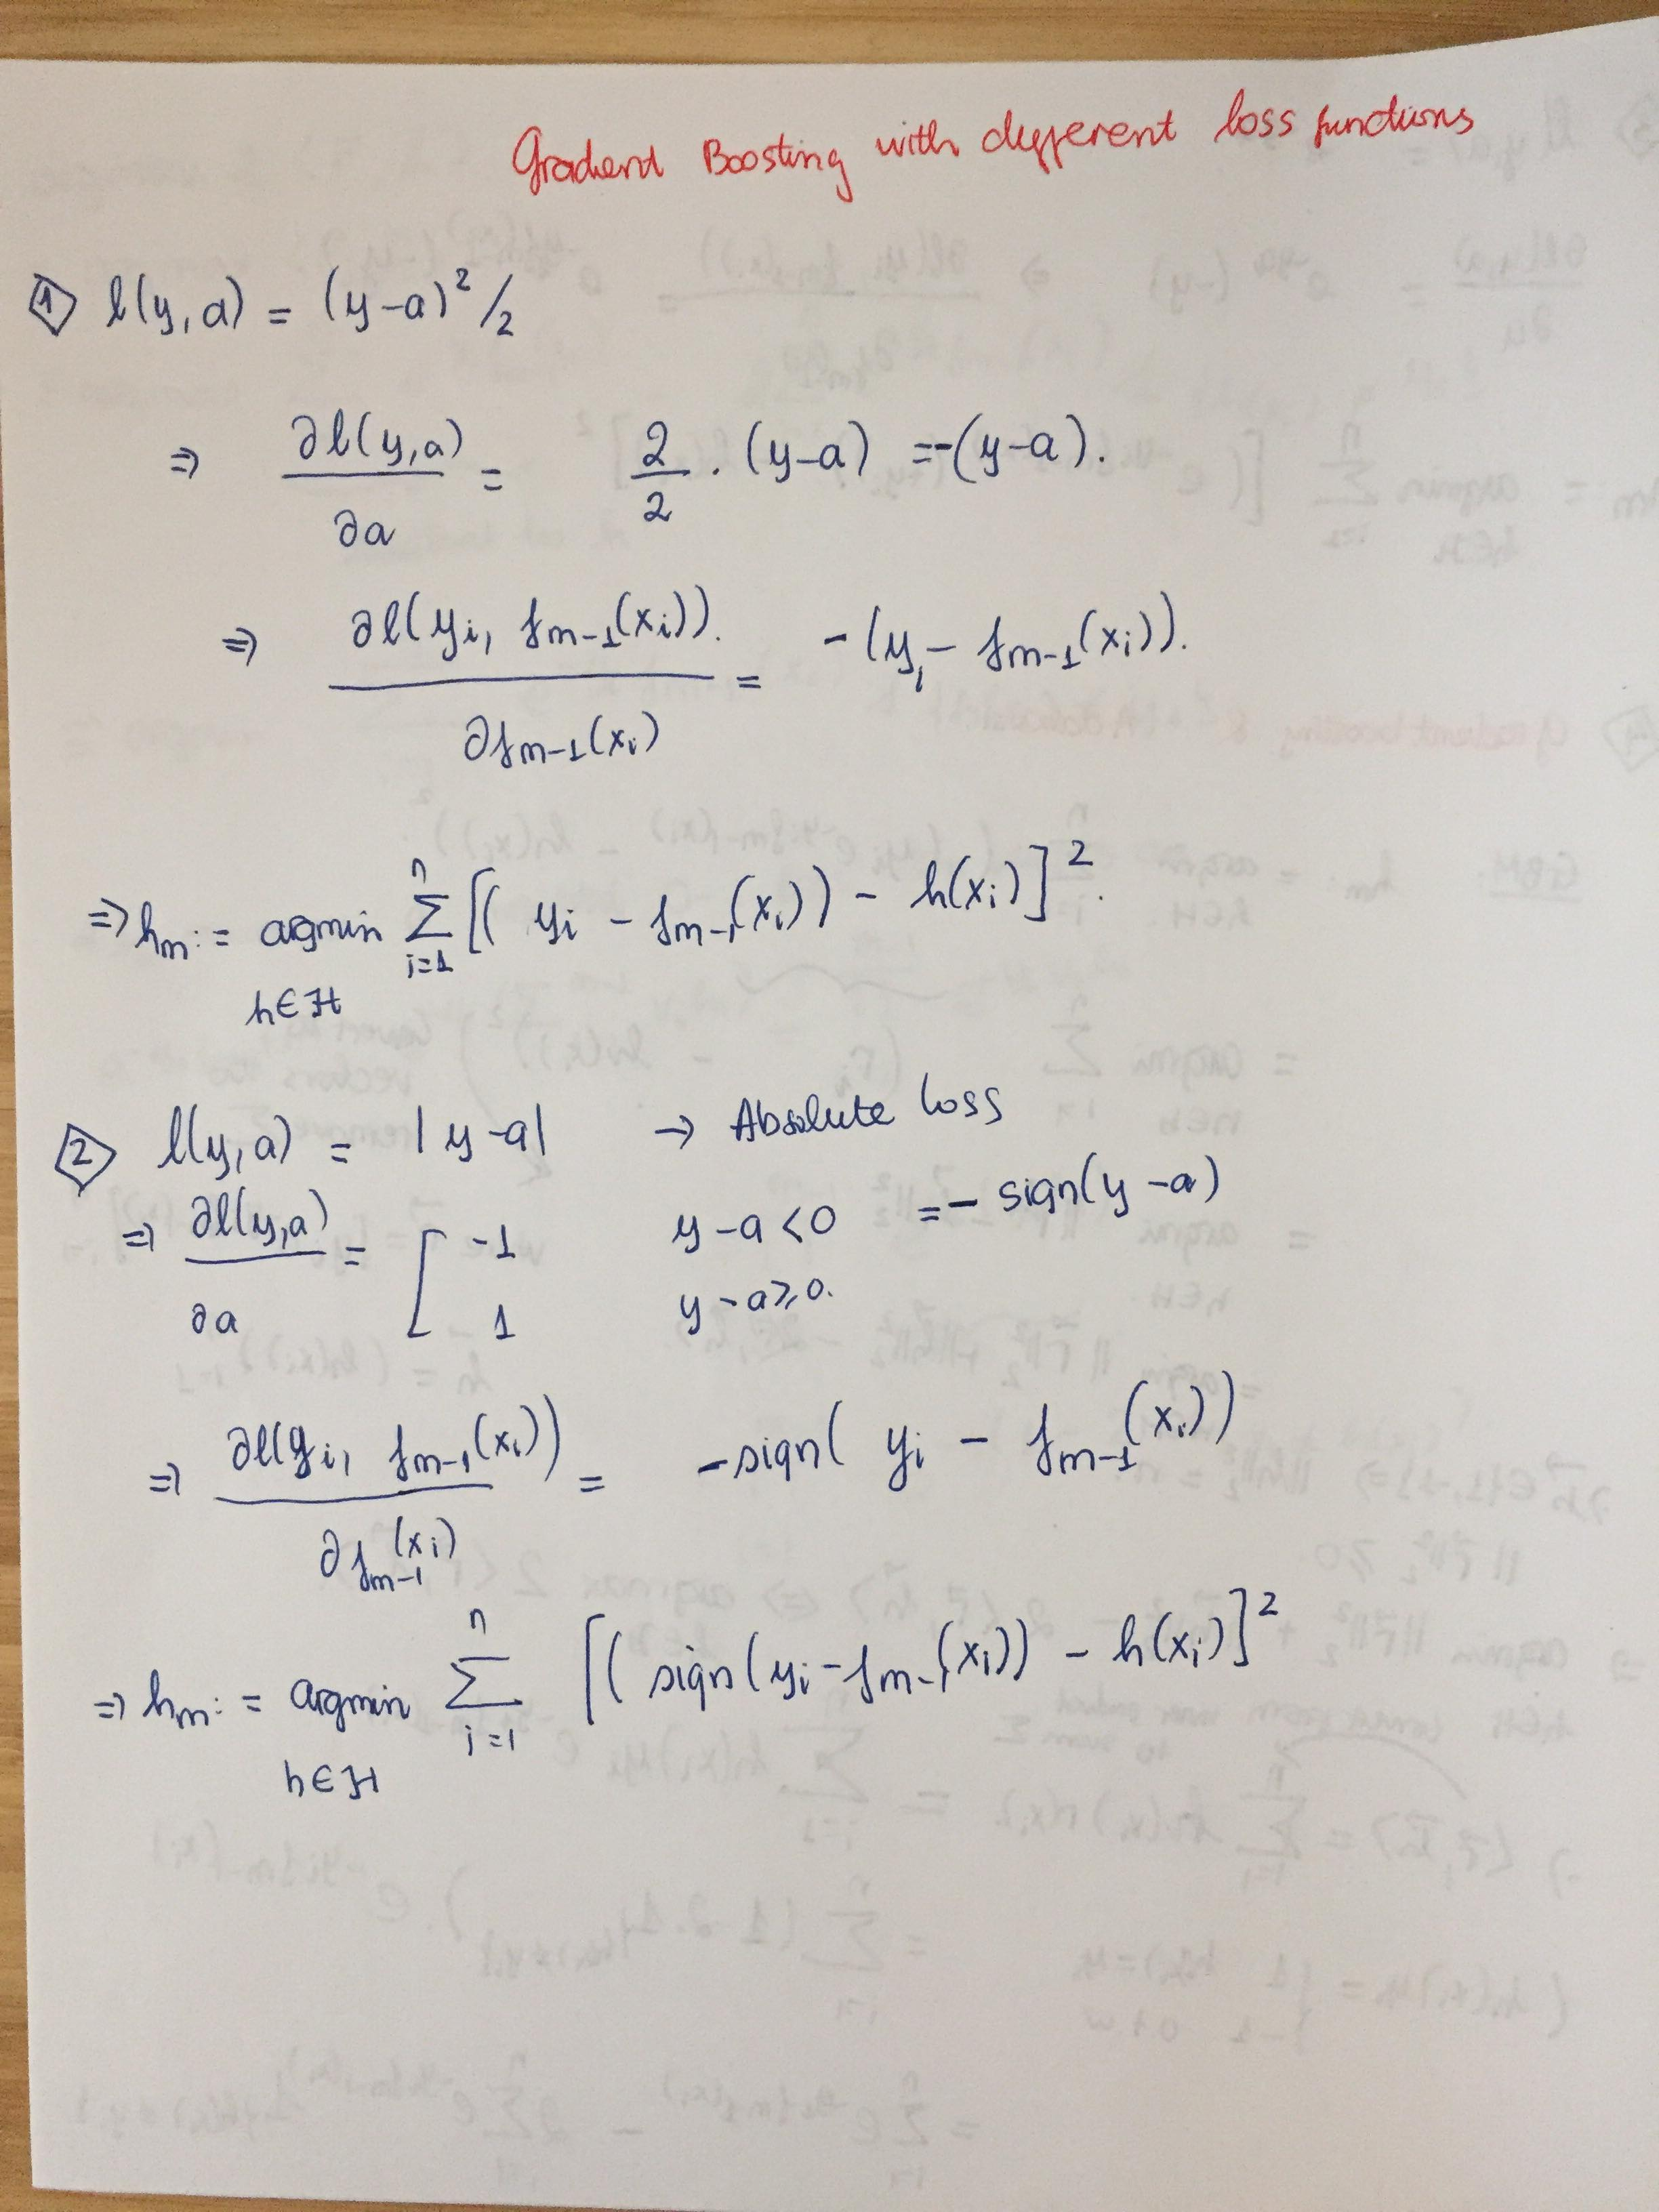
\includegraphics[max size={\textwidth}{0.9\textheight}]{GBM3.jpg} \\

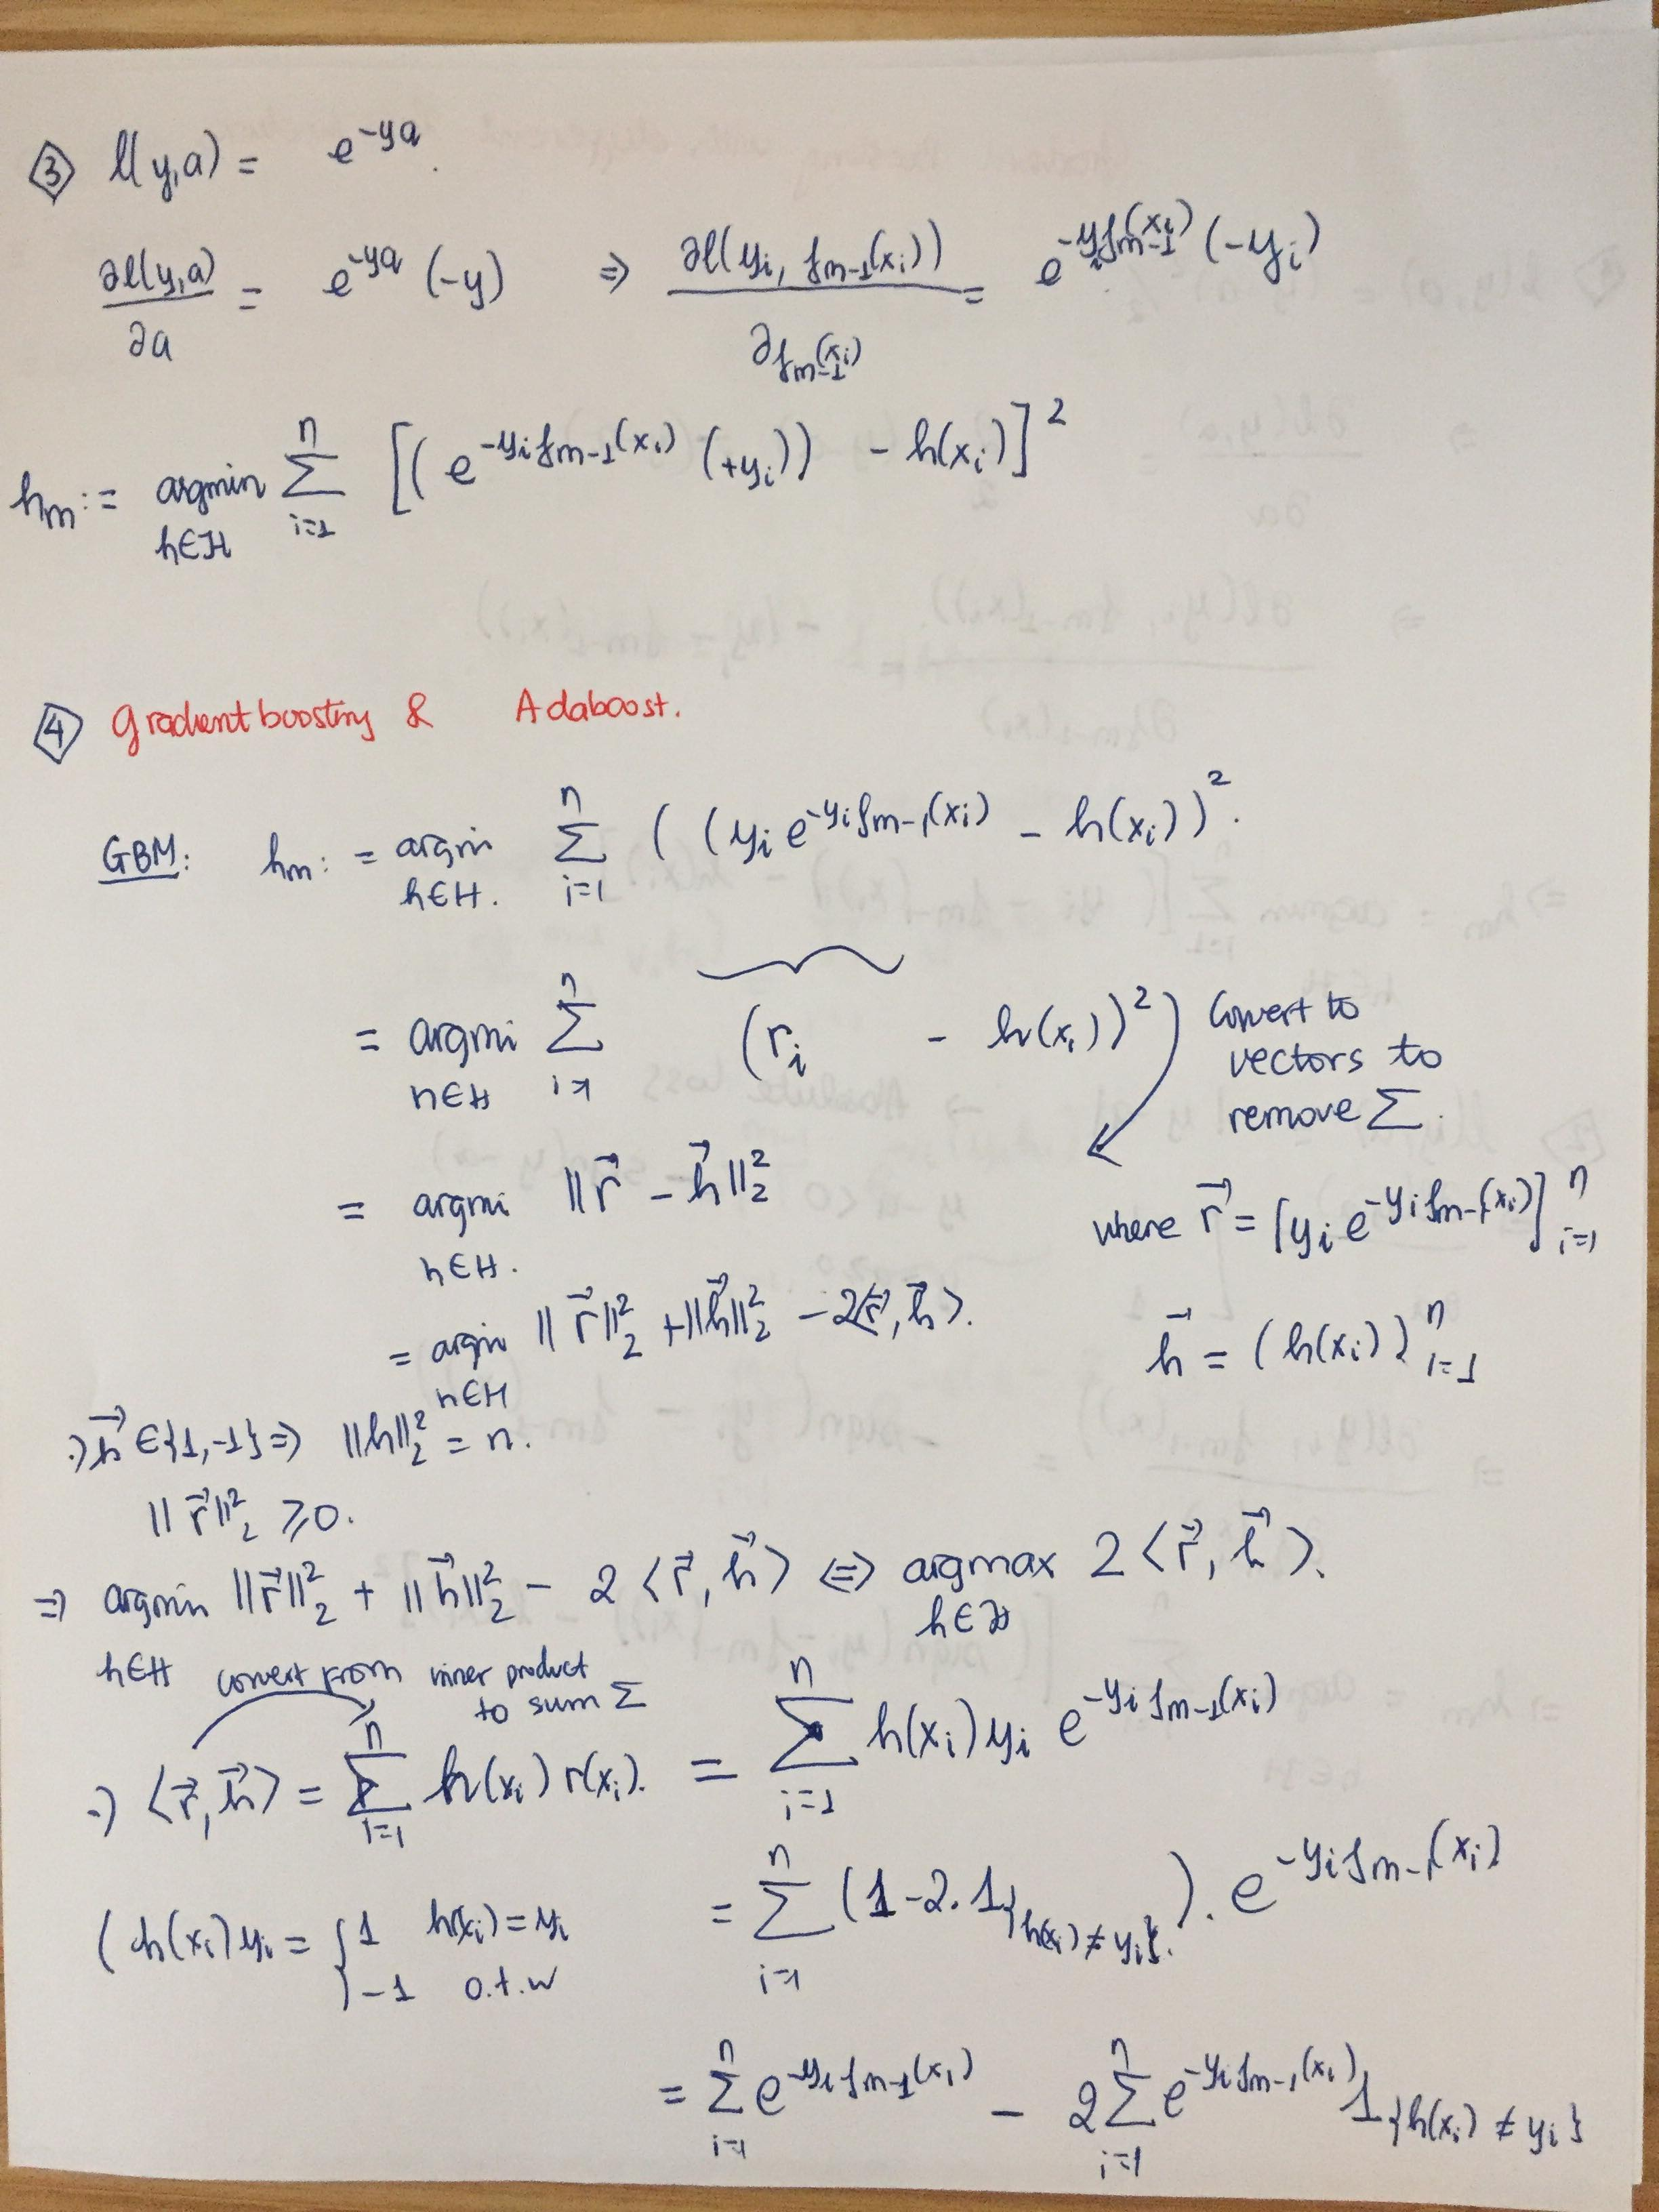
\includegraphics[max size={\textwidth}{0.9\textheight}]{GBM4.jpg} \\

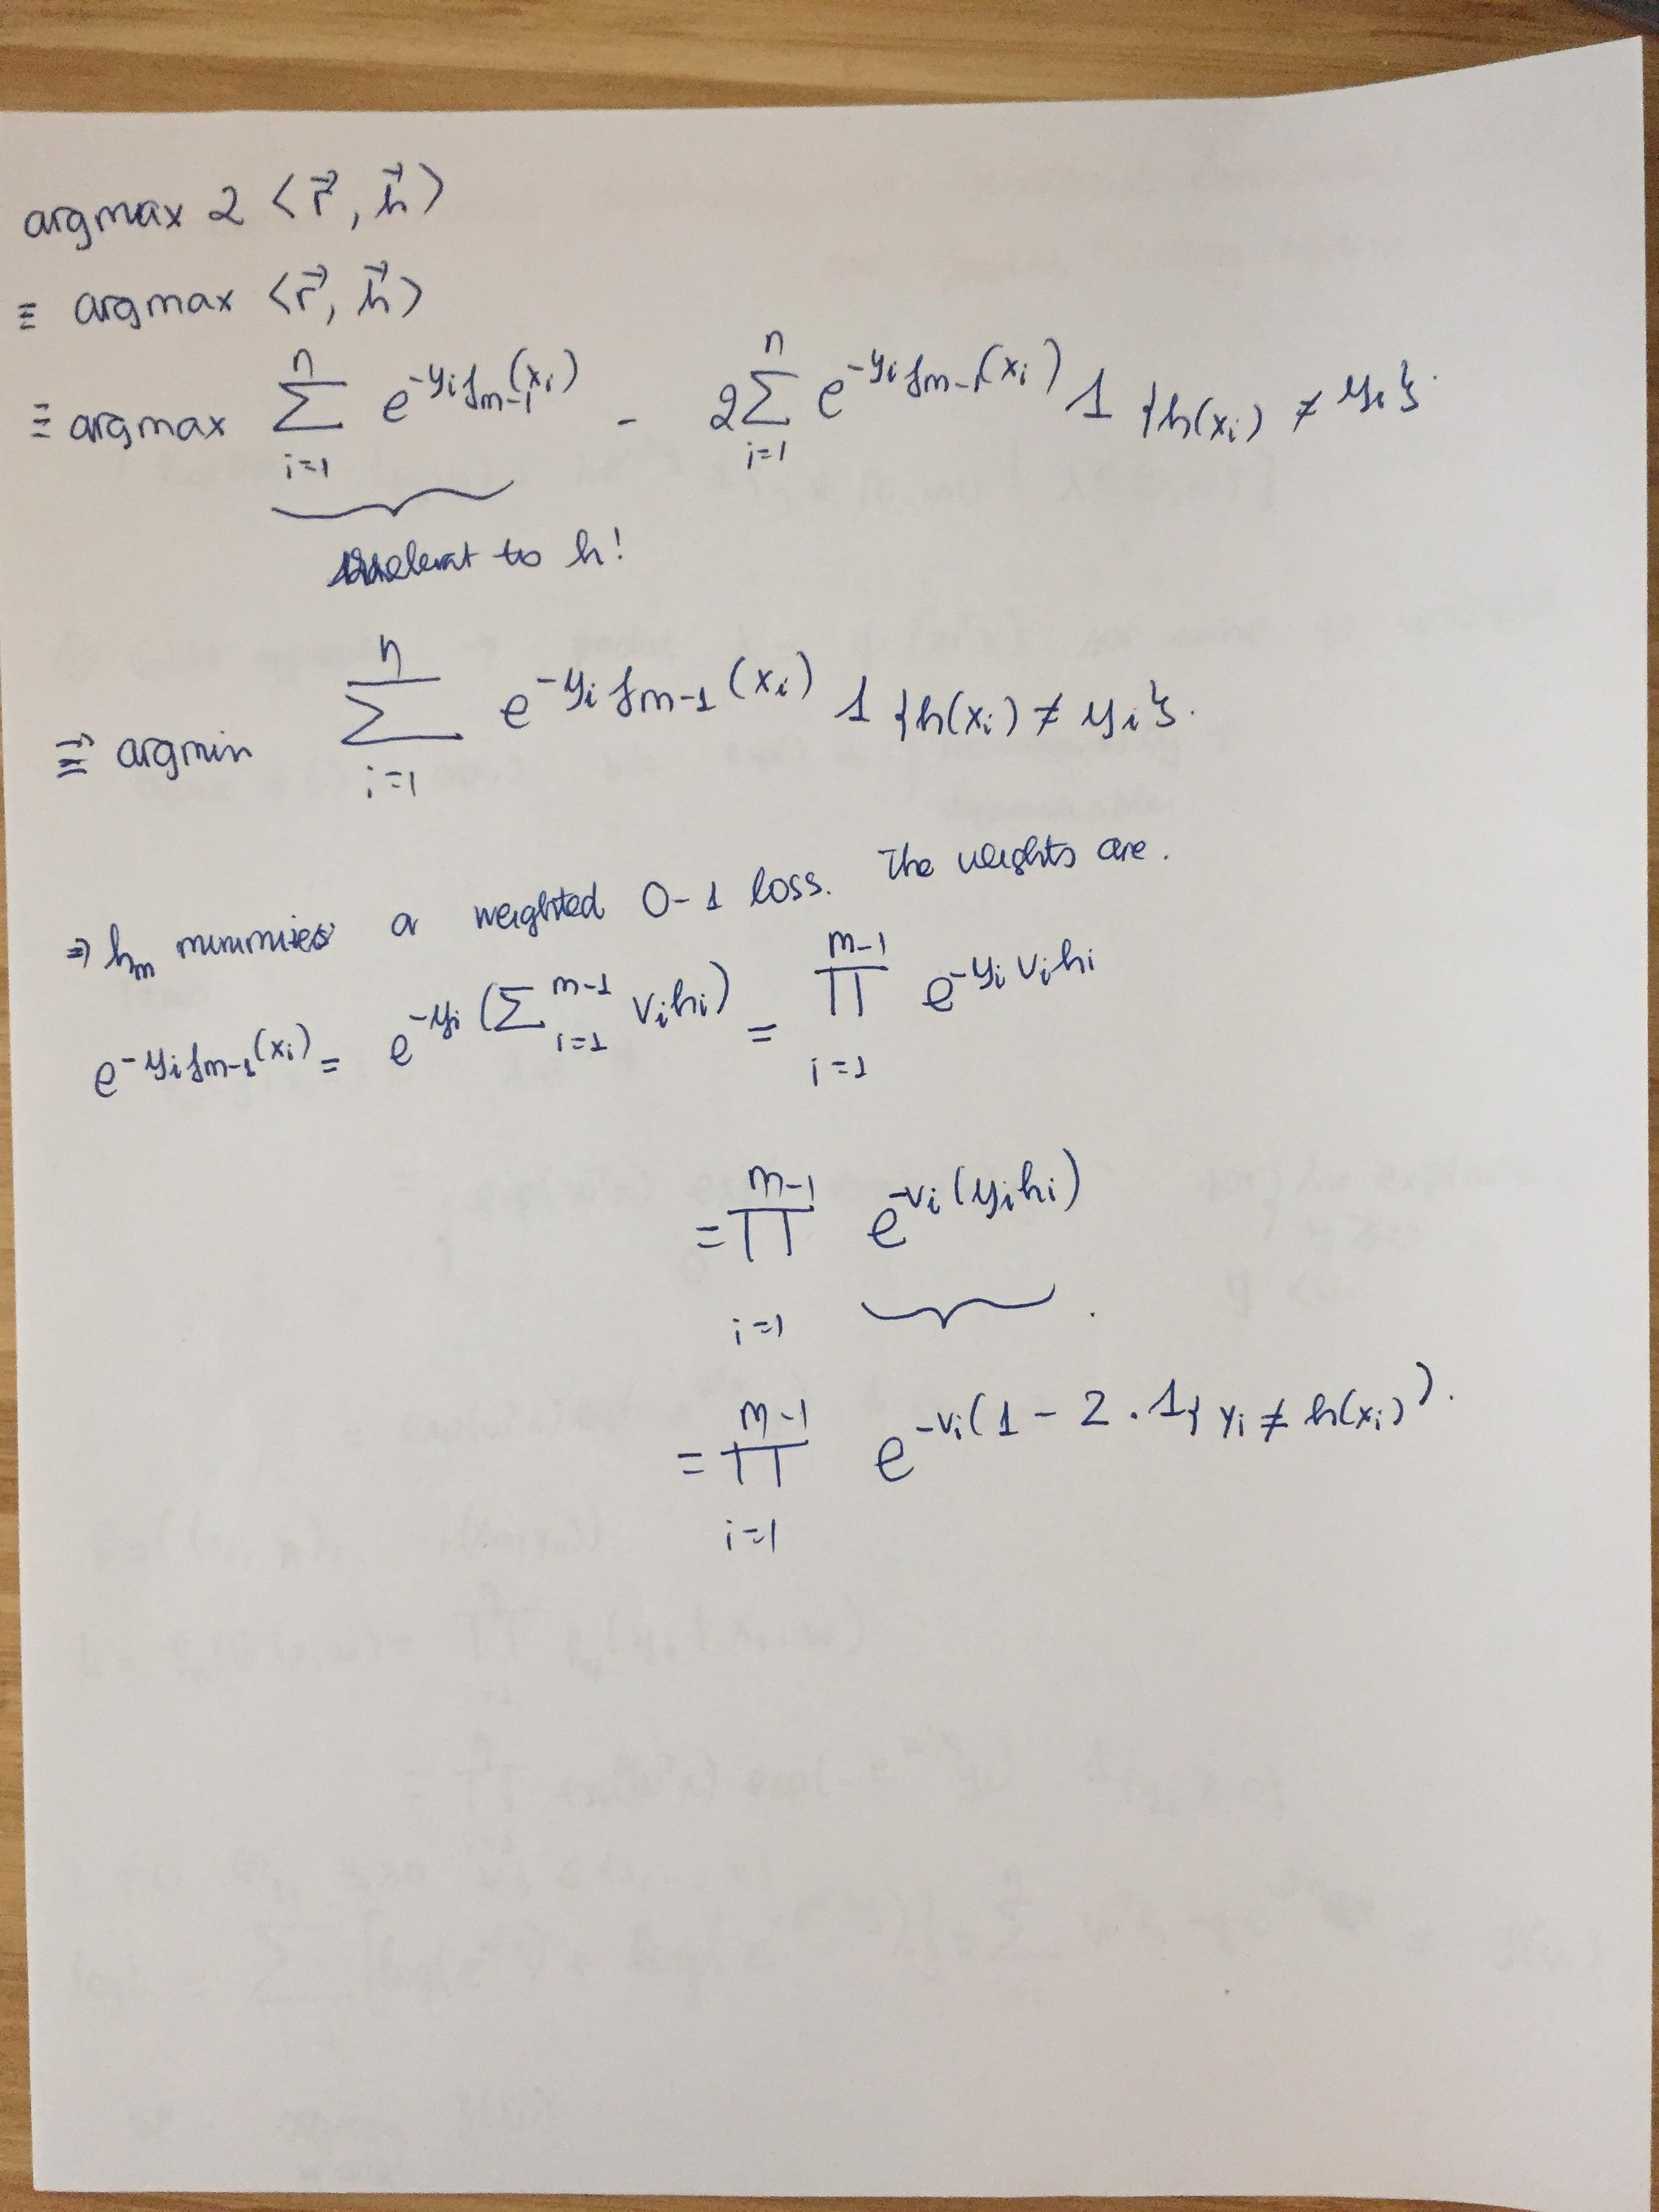
\includegraphics[max size={\textwidth}{0.9\textheight}]{GBM5.jpg} \\


\end{document}
